\chapter{SOI増幅器を用いたSTJ信号増幅試験}
	\section{測定素子}
		\subsection{Nb/Al-STJ検出器}
			本測定では産業技術総合研究所(AIST)のCRAVITY製のNb/Al-STJ検出器を使用した。
			用いたNb/Al-STJ検出器の各層の厚みを表\ref{tab:NbAlSTJ_detail}に示す。
			\begin{table}[htb]
				\begin{center}
					\begin{tabular}{| l | c |} \hline
						\  & 厚さ[$\mathrm{nm}$] \\ \hline \hline
						上部ニオブ層 & 100 \\ \hline
						上部アルミニウム層 & 70 \\ \hline
						アルミナ$\mathrm{Al_{2}O_{3}}$ & 1 \\ \hline
						下部アルミニウム層 & 70 \\ \hline
						下部ニオブ層 & 100 \\ \hline
					\end{tabular}
					\caption{増幅試験に用いたSTJ検出器の厚さ}
					\label{tab:NbAlSTJ_detail}
				\end{center}
			\end{table}
			
			このSTJ検出器のマスクデザインを図\ref{fig:NbAlSTJ_mask}に示す。
			STJ信号増幅に用いたNb/Al-STJ検出器は図\ref{fig:NbAlSTJ_mask}の「Division3」に属する20$\mathrm{\mu m}$角のNb/Al-STJ検出器を用いた。
			
			\begin{figure}[htbp]
				\begin{center}
					\includegraphics[width=12.0cm]{./Chapter/Chapter4/Picture/NbAlSTJ_mask.eps}
					\caption{産総研CRAVITY製Nb/Al-STJ検出器\ マスクデザイン}
					\label{fig:NbAlSTJ_mask}
				\end{center}
			\end{figure}
		
			\clearpage
	\section{測定環境}
		\subsection{$\mathrm{^{3}He}$減圧冷凍機}
			\subsubsection{構造}
				我々はNb/Al-STJ検出器を300mK環境下で動作させるために、$\mathrm{^{3}He}$減圧冷凍機を用いて素子の冷却を行った。
				本研究に使用している$\mathrm{^{3}He}$減圧冷凍機は、Oxford Instruments社 HelioxAC-V $\mathrm{^{3}}$He Refrigeratorである。
				この$\mathrm{^{3}He}$減圧冷凍機は$\mathrm{^{3}He}$を減圧することによって冷却し、約300mK程度までの冷却を行うことができる。
								
				\begin{figure}[htbp]
					\begin{center}
						\begin{tabular}{c}
							%1
							\begin{minipage}{0.6\hsize}
								\begin{center}
									\includegraphics[clip, width=8cm]{./Chapter/Chapter4/Picture/He3_sorption_stage.eps}
									\hspace{1.6cm} [a]外観
								\end{center}
							\end{minipage}
							%2
							\begin{minipage}{0.4\hsize}
								\begin{center}
									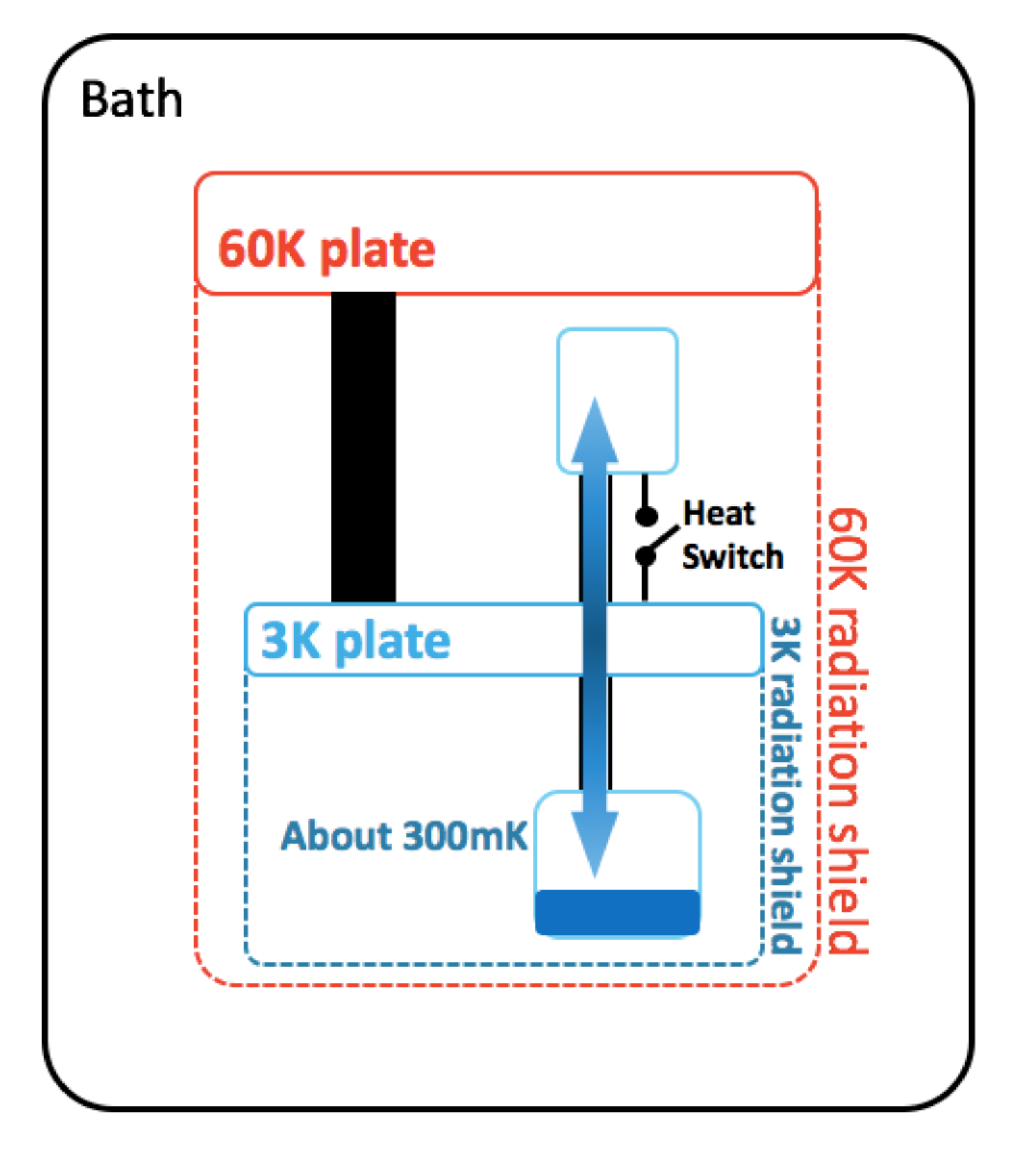
\includegraphics[clip, width=4cm]{./Chapter/Chapter4/Picture/He3sorption_structure.eps}
									\hspace{1.6cm} [b]構造概念図
								\end{center}
							\end{minipage}
						\end{tabular}
						\caption{$\mathrm{^{3}He}$減圧冷凍機}
						\label{fig:He3sorption}
					\end{center}
				\end{figure}
				
				この冷凍機の冷却能力について、表\ref{tab:He3_sorption}に各ステージごとにまとめた。
				60Kステージ、3Kステージそれぞれには熱輻射シールドを設置している。
				またNb/Al-STJ検出器に外部から磁場が侵入しないようにパーマロイテープと呼ばれる磁場シールドも設置している。
				\begin{table}[htb]
					\begin{center}
						\begin{tabular}{| l | c | l |} \hline
							ステージ & 到達温度[K] & 冷却能力 \\ \hline
							60K & 60K & 25W\ @65K \\
							3K & 2.8K & 0.7W\ @4.2K \\
							最低温 & 0.3K & 100$\mathrm{\mu W}$\ @350mK \\ \hline
						\end{tabular}
						\caption{$\mathrm{^{3}He}$減圧冷凍機\ 各ステージの到達温度と冷却能力}
						\label{tab:He3_sorption}
					\end{center}
				\end{table}
				
				\clearpage
			
			\subsubsection{動作原理}
				\begin{figure}[htbp]
					\begin{center}
						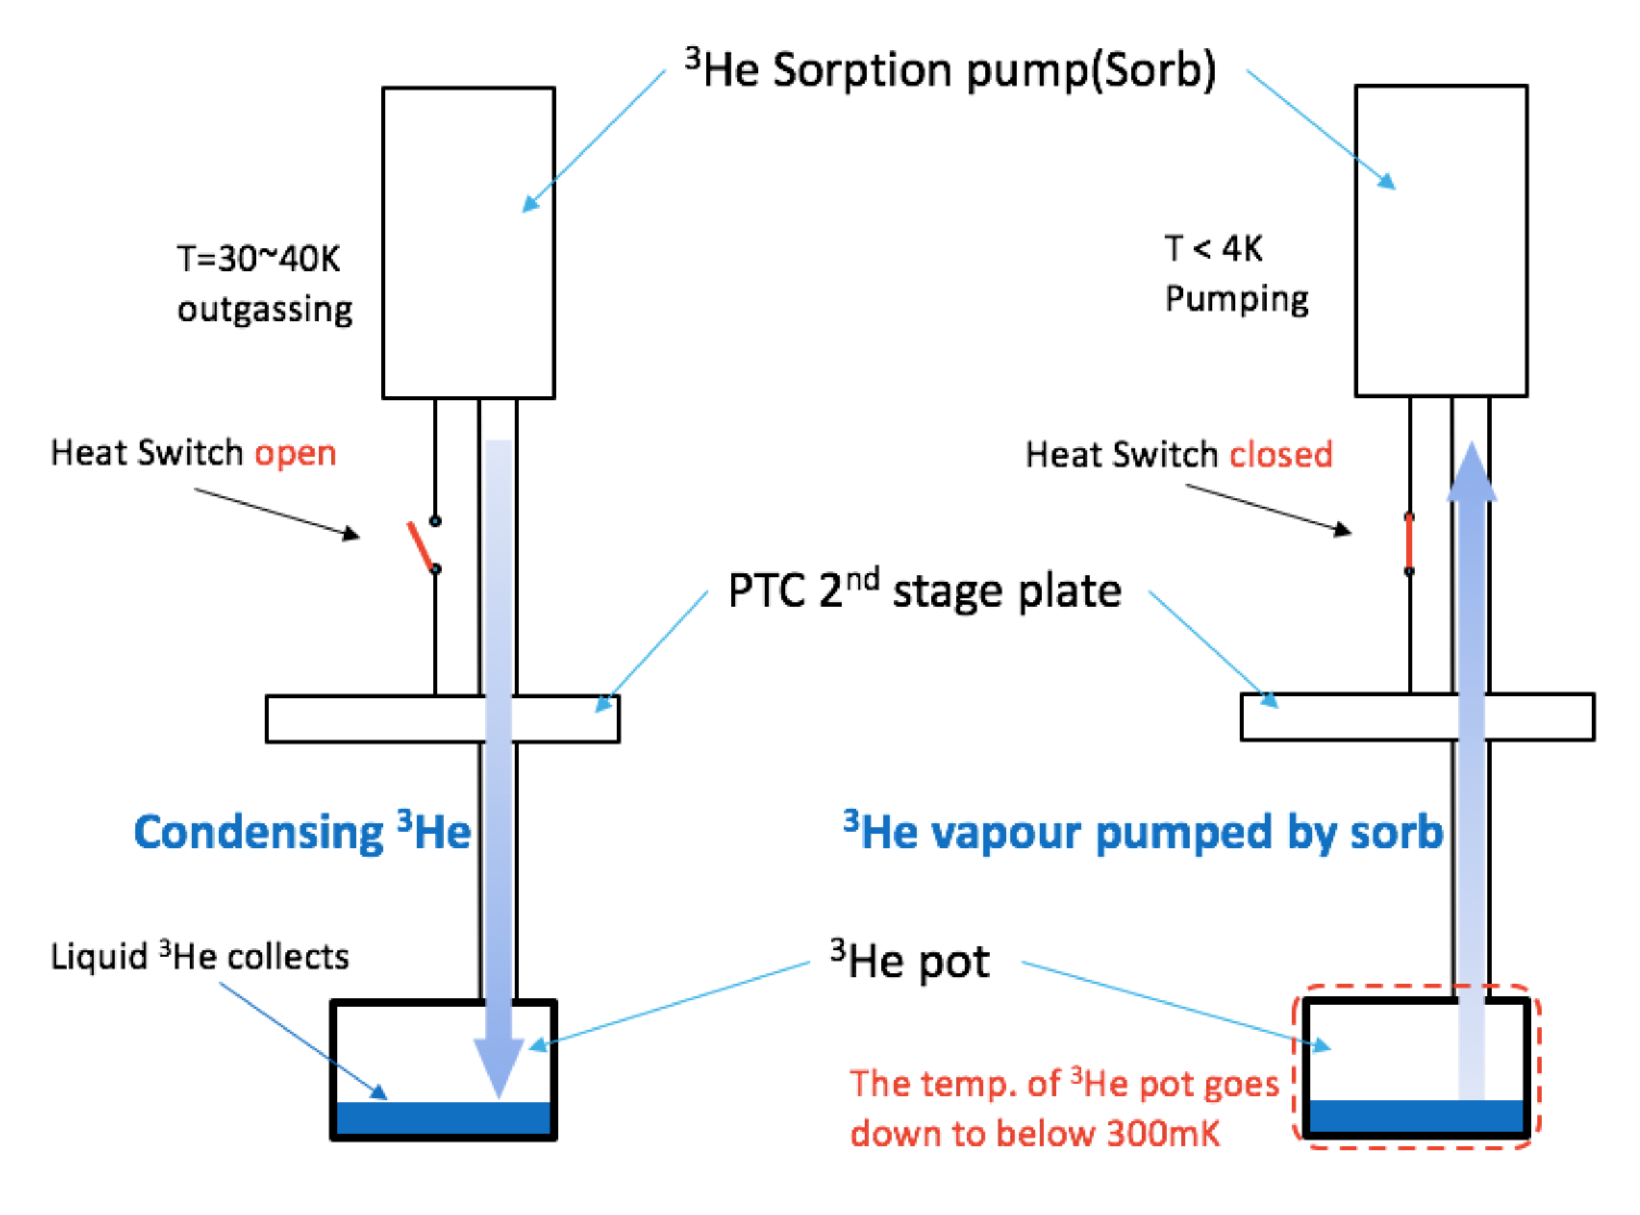
\includegraphics[width=12.0cm]{./Chapter/Chapter4/Picture/He3sorption.eps}
						\caption{$\mathrm{^{3}He減圧冷凍機\ 動作概念図}$}
						\label{fig:He3sorption}
					\end{center}
				\end{figure}
				図\ref{fig:He3sorption}に$\mathrm{^{3}He}$減圧冷凍機の動作概念図を示した。
				まず、パルスチューブ冷凍機を用いて室温から3K程度まで冷却を行う。
				その後、図\ref{fig:He3sorption}のHeatSwitchを接続(close)することで、SorbとPTC 2nd Plateを熱伝導させることで3Kに冷却される。
				Sorbは冷却されることにより、Sorbには$\mathrm{^{3}He}$が吸着される。
				
				その後、HeatSwitchによる接続を解除(open)し、Sorbに付属しているHeaterで30K程度になるように熱を加える。
				すると、図\ref{fig:He3sorption}の左図のように、Sorbに吸着されていた$\mathrm{^{3}He}$が液化し、それが$\mathrm{^{3}He}$\ potに溜まる。
				そして、$\mathrm{^{3}He}$の液化後、SorbのHeaterの出力を止め、HeatSwitchによる接続(close)を行い、Sorbの冷却を再度行う。
				これにより、図\ref{fig:He3sorption}の右図のように、$\mathrm{^{3}He}$ potに溜まっている$\mathrm{^{3}He}$をSorbに吸着させることで、$\mathrm{^{3}He}$が減圧冷凍され、3Kから300mK程度までの冷凍がスタートする。
				\clearpage
	
	\section{SOI増幅器を用いたsin波増幅試験}
		我々は昨年度SOI-STJ4についての性能評価を行い、極低温環境下でSTJ検出器の信号を十分増幅可能な回路を設計できたと結論付けた。
		この結果を受け、我々は極低温環境下でSOI増幅器を用いたSTJ検出器信号の増幅試験を行った。
		
		そこで、まず我々はSTJ信号増幅の前にSOI-STJ4とNb/Al-STJを接続した回路であっても、SOI-STJ4が動作するかを確認するためにsin波増幅試験を行った。
		\subsection{SOI-STJ4のみのsin波増幅試験}
			\begin{figure}[htbp]
				\begin{center}
					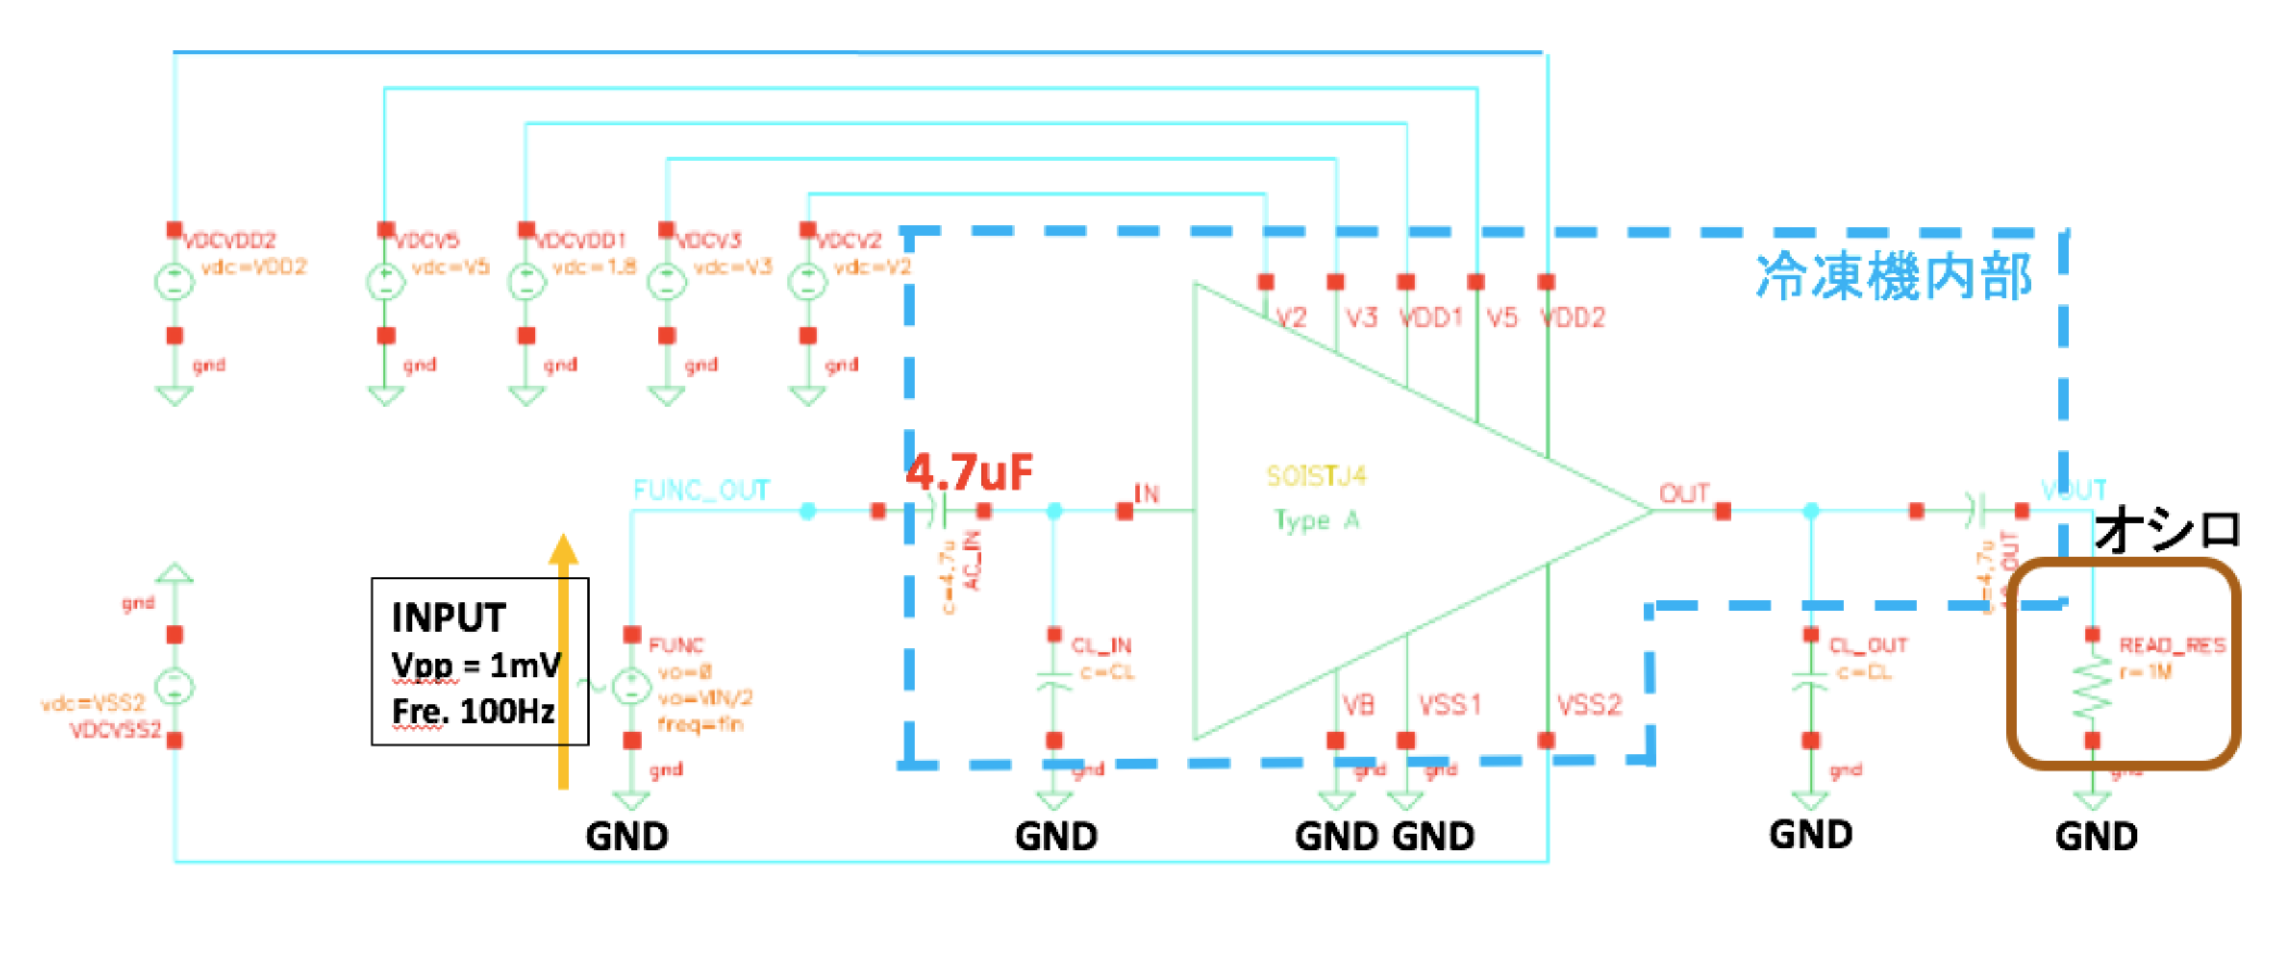
\includegraphics[width=12.0cm]{./Chapter/Chapter4/Picture/SOISTJ4woSTJ_amp_sin.eps}
					\caption{SOI-STJ4のみを用いたsin波増幅試験\ 回路図}
					\label{fig:SOISTJ4woSTJ_amp_sin}
				\end{center}
			\end{figure}
			図\ref{fig:SOISTJ4woSTJ_amp_sin}にSOI-STJ4のみを用いたsin波増幅試験の回路図を示した。
			sin波入力にはFunction Generatorを用いており、周波数を走査させながら、出力波形を測定した。
			出力波形が飽和しないように、入力sin波の波高はpeak\ to\ peakで1mVとした。
			Function GeneratorとSOI-STJ4の入力端子との間には、常温環境下で4.7$\mathrm{\mu F}$の積層型セラミックコンデンサーを介し、AC的に接続をした。
			
			入出力波形はオシロスコープで読み取った。オシロスコープの設定は、
			\begin{itemize}
				\item 入力インピーダンス\ $1\mathrm{M \Omega}$
				\item AC結合
				\item 512回平均
			\end{itemize}
			である。
			入出力それぞれの波高(peak\ to\ peak)を取得し、利得Gainを式(\ref{eq:gain_definition})のように定義した。
			\begin{eqnarray}
				\mathrm{Gain} = \frac{V_{\mathrm{peak\ to\ peak}}(\mathrm{OUTPUT})}{V_{\mathrm{peak\ to\ peak}}(\mathrm{INPUT})}
				\label{eq:gain_definition}
			\end{eqnarray}
			
			\clearpage
			入力周波数が100Hzのとき、1MHzのとき、それぞれの入出力波形を図\ref{fig:SOISTJ4woSTJ_InOut_100Hz}と図\ref{fig:SOISTJ4woSTJ_InOut_1MHz}に示した。
			それぞれ黄線が入力波形、青線が出力波形を示す。
			
			まず$f_{\mathrm{input}=100\mathrm{Hz}}$のときの図\ref{fig:SOISTJ4woSTJ_InOut_100Hz}を見ると、入力に対し出力の位相が180度ずれて反転増幅していることがわかる。
			利得は約100程度である。
			対して、$f_{\mathrm{input}=1\mathrm{MHz}}$のときの図\ref{fig:SOISTJ4woSTJ_InOut_1MHz}を見ると、100Hzのときと比べると位相がずれて増幅されているのがわかる。
			そして利得は約30程度に下がっている。
			
			利得の周波数特性を示した図を図\ref{fig:SOISTJ4woSTJ_frequency}に示す。
			SOI-STJ4は入力周波数100kHz程度までは利得は落ちることなく増幅可能である。
			100kHzを超え始めると次第に利得は減少するが、冷凍機読み出し配線容量0.5nF、1MHz\ sin波に対し利得約30程度を獲得した。
			
			STJ検出器信号の速度が約$1\mathrm{\mu s}$であることからSTJ検出器信号を十分増幅できると示唆する結果を示せた。
			しかし、このときのSOI-STJ4の消費電力は$230\mathrm{\mu W}$で、最低温ステージ環境下での冷凍機の冷却能力を上回ってしまう。
			実際、SOI-STJ4の動作中の最低温ステージの温度は約300mKから約500から600mK程度まで上昇していた。
			この温度領域ではNb/Al-STJ検出器の熱雑音が落ちきらない。
			
			本実験では、SOI-STJ4を用いてのSTJ検出器信号を増幅させることが目的である。
			もしSOI-STJ4の動作によってNb/Al-STJ検出器が600mK程度までの温度上昇しても、Nb/Al-STJ検出器は超伝導検出器として動作する。
			したがって、本実験での200mK程度の温度上昇を問題としないこととする
			\footnote{我々はNb/Al-STJ検出器を熱起因雑音が落ちきる300mK環境下で動作させたいが、最低温ステージの冷却能力以下の消費電力で極低温前置増幅器を動作させるのは現状厳しい。そこで我々はSOI前置増幅器を3Kステージに設置し増幅させることを考えている。}。
			
			\begin{figure}[htbp]
				\begin{center}
					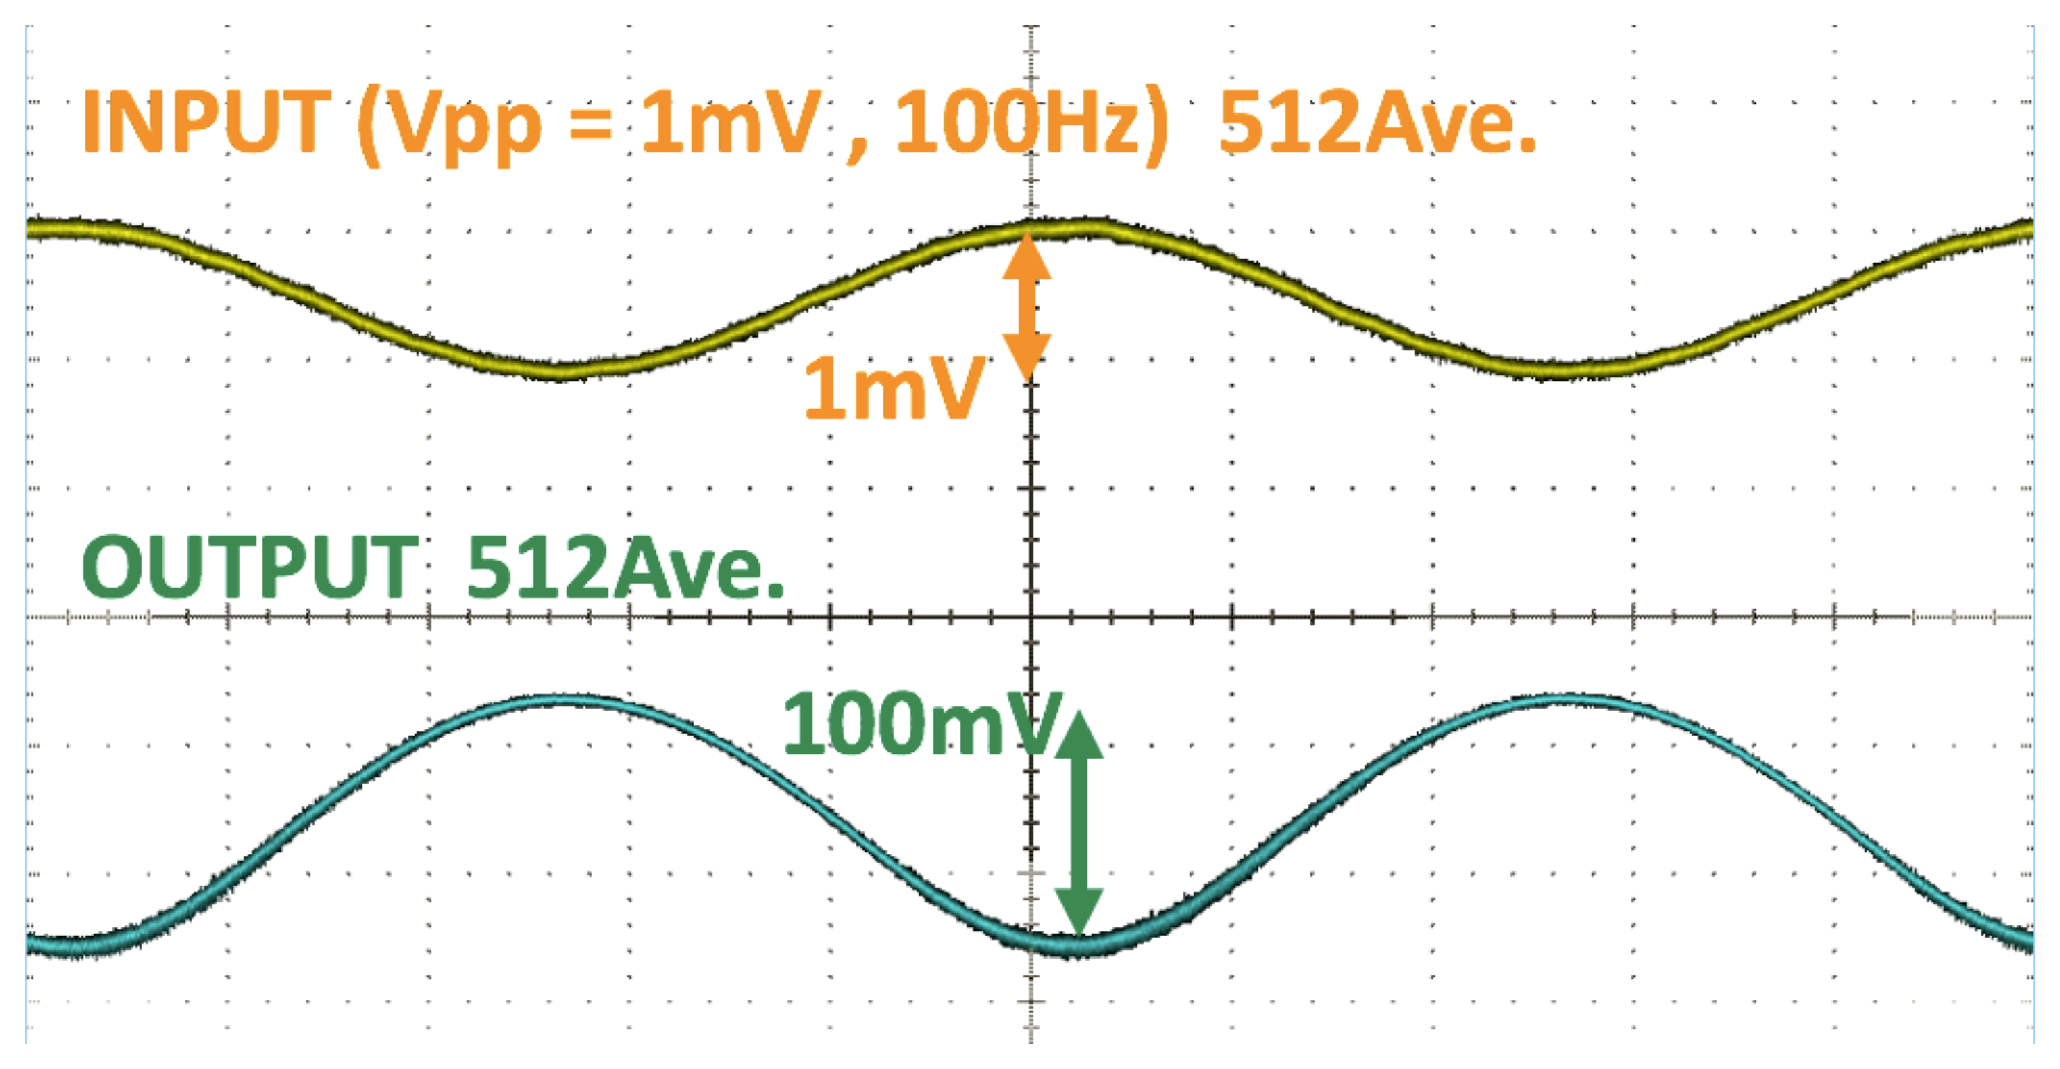
\includegraphics[width=12.0cm]{./Chapter/Chapter4/Picture/SOISTJ4woSTJ_InOut_100Hz.eps}
					\caption{SOI-STJ4のみを用いたsin波増幅試験\ 入出力波形($f_{\mathrm{input}}=100\mathrm{Hz}$)}
					\label{fig:SOISTJ4woSTJ_InOut_100Hz}
				\end{center}
			\end{figure}
			\begin{figure}[htbp]
				\begin{center}
					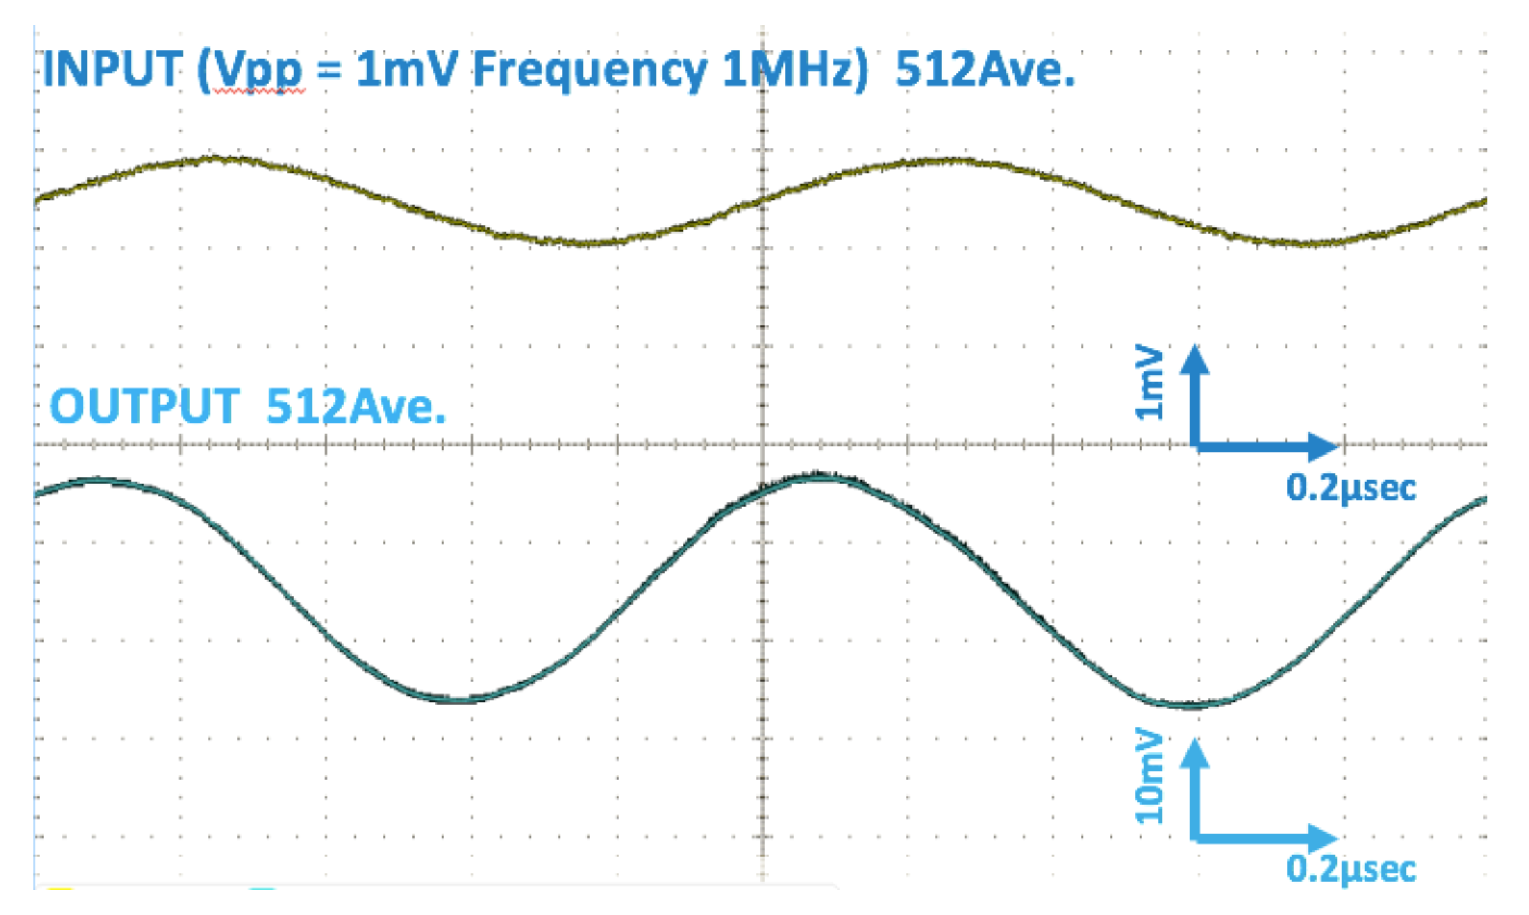
\includegraphics[width=12.0cm]{./Chapter/Chapter4/Picture/SOISTJ4woSTJ_InOut_1MHz.eps}
					\caption{SOI-STJ4のみを用いたsin波増幅試験\ 入出力波形($f_{\mathrm{input}}=100\mathrm{Hz}$)}
					\label{fig:SOISTJ4woSTJ_InOut_1MHz}
				\end{center}
			\end{figure}
			
			\begin{figure}[htbp]
				\begin{center}
					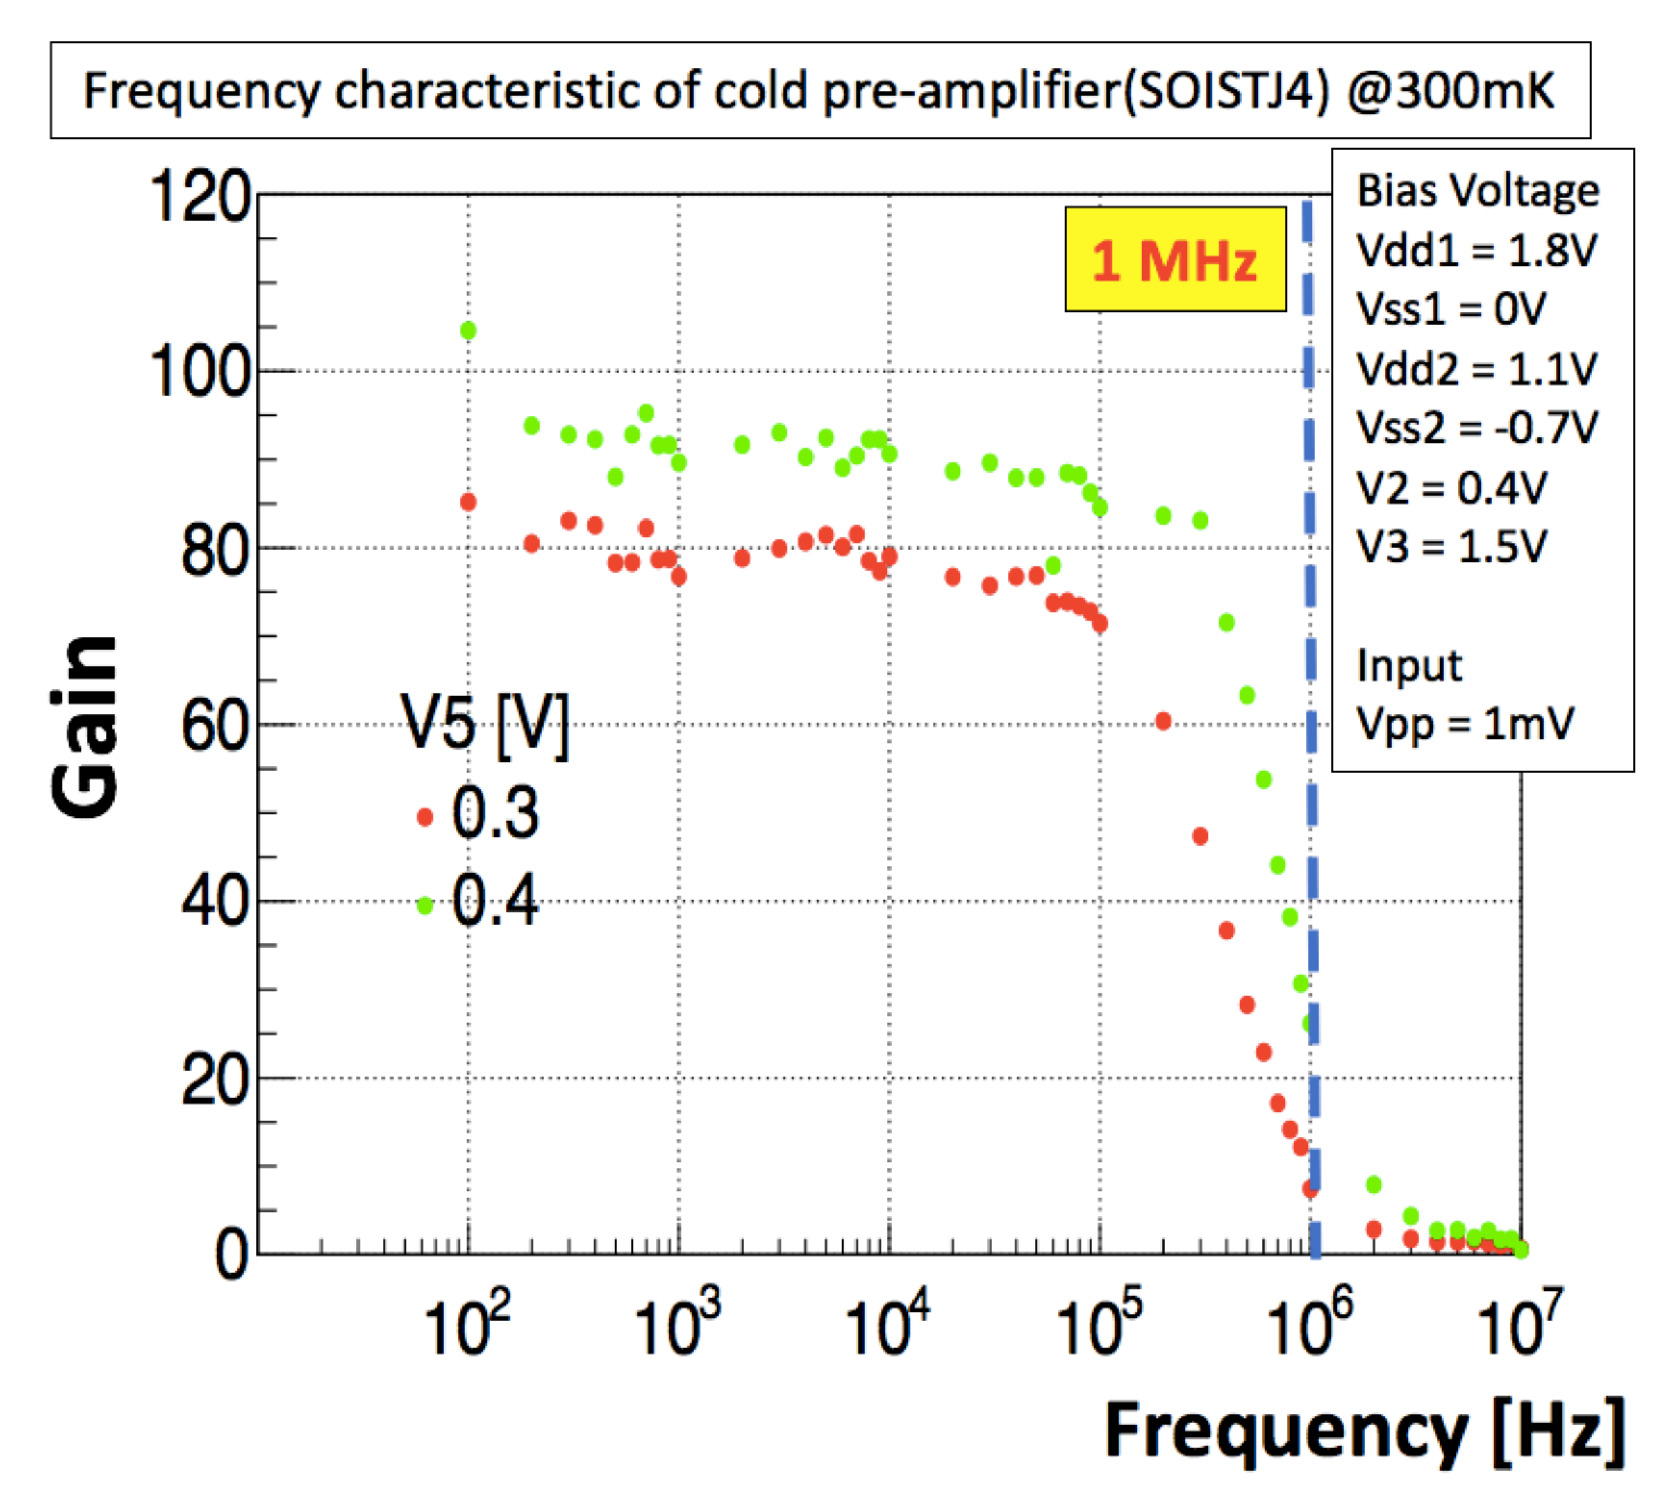
\includegraphics[width=12.0cm]{./Chapter/Chapter4/Picture/SOISTJ4woSTJ_frequency.eps}
					\caption{SOI-STJ4のみを用いたsin波増幅試験\ 利得の周波数依存性}
					\label{fig:SOISTJ4woSTJ_frequency}
				\end{center}
			\end{figure}
			\clearpage
			
		
		\subsection{Nb/Al-STJ検出器と組み合わせた回路でのSOI-STJ4を用いたsin波増幅試験}
			\begin{figure}[htbp]
				\begin{center}
					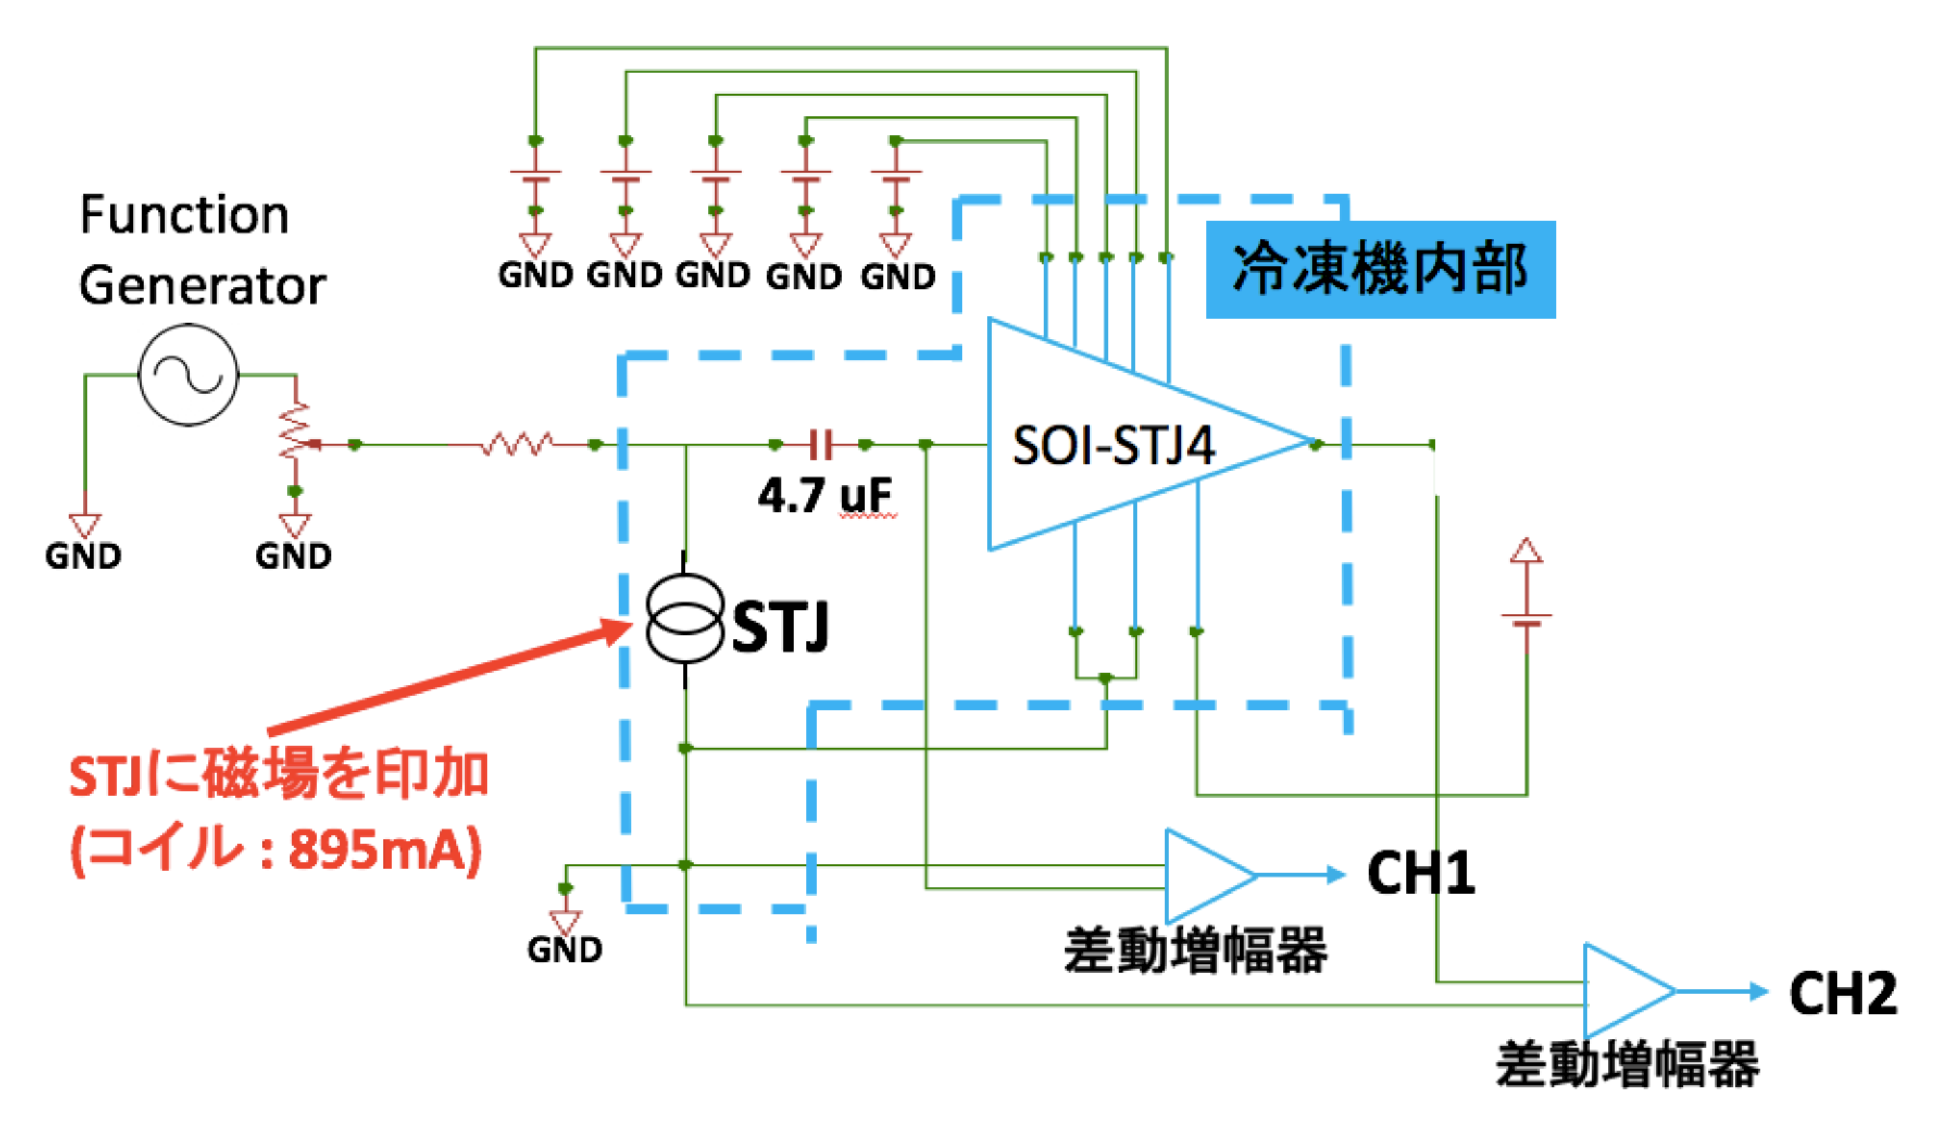
\includegraphics[width=12.0cm]{./Chapter/Chapter4/Picture/SOISTJ4wSTJ_amp_sin.eps}
					\caption{Nb/Al-STJ検出器と組み合わせた回路でのSOI-STJ4を用いたsin波増幅試験\ }
					\label{fig:SOISTJ4wSTJ_amp_sin}
				\end{center}
			\end{figure}
			300mK環境下におけるSOI-STJ4単体でのsin波増幅試験の結果、読み出し配線容量0.5nF、1MHz\ sin波に対して利得約30程度を観測した。
			次に、我々はNb/Al-STJ検出器と組み合わせた回路でSOI-STJ4のsin波増幅試験を行い、SOI-STJ4が前節と同様の性能を示すかを確かめる。
			図\ref{fig:SOISTJ4wSTJ_amp_sin}はNb/Al-STJ検出器と組み合わせた回路でのSOI-STJ4を用いたsin波増幅試験の回路図を示す。
			極低温環境下においてSTJ検出器の両端電圧を印加しなくてもジョセフソン電流が回路に流れてしまう。
			本測定ではジョセフソン電流を抑制するために磁場を印加しながら測定した。
			
			入力sin波、オシロスコープの設定は前節と同様の設定で行い、sin波の周波数を走査させながら入出力波形をオシロスコープで読み取った。
			
			入力sin波周波数$f_{\mathrm{input}}=100\mathrm{Hz}$のときの入出力波形を図\ref{fig:SOISTJ4wSTJ_InOut_100Hz}に示す。
			このときSOI-STJ4単体の場合と同様に利得97の反転増幅を観測した。
			そして、入力sin波周波数$f_{\mathrm{input}}=1\mathrm{MHz}$のときの入出力波形を図\ref{fig:SOISTJ4wSTJ_InOut_1MHz}に示す。
			この場合もSOI-STJ4単体の場合と同様に、入力波形と出力波形の位相はずれており、利得40程度の反転増幅を観測した。
			
			Nb/Al-STJ検出器を組み合わせた回路での利得の周波数特性を図\ref{fig:SOISTJ4wSTJ_frequency}に示す。
			SOI-STJ4単体の場合の利得の周波数依存性を示した図\ref{fig:SOISTJ4woSTJ_frequency}と同様の周波数特性を示していた。
			このことから、Nb/Al-STJ検出器と組み合わせてもSOI-STJ4は単体と同様の性能を示したことになる。
			
			\begin{figure}[htbp]
				\begin{center}
					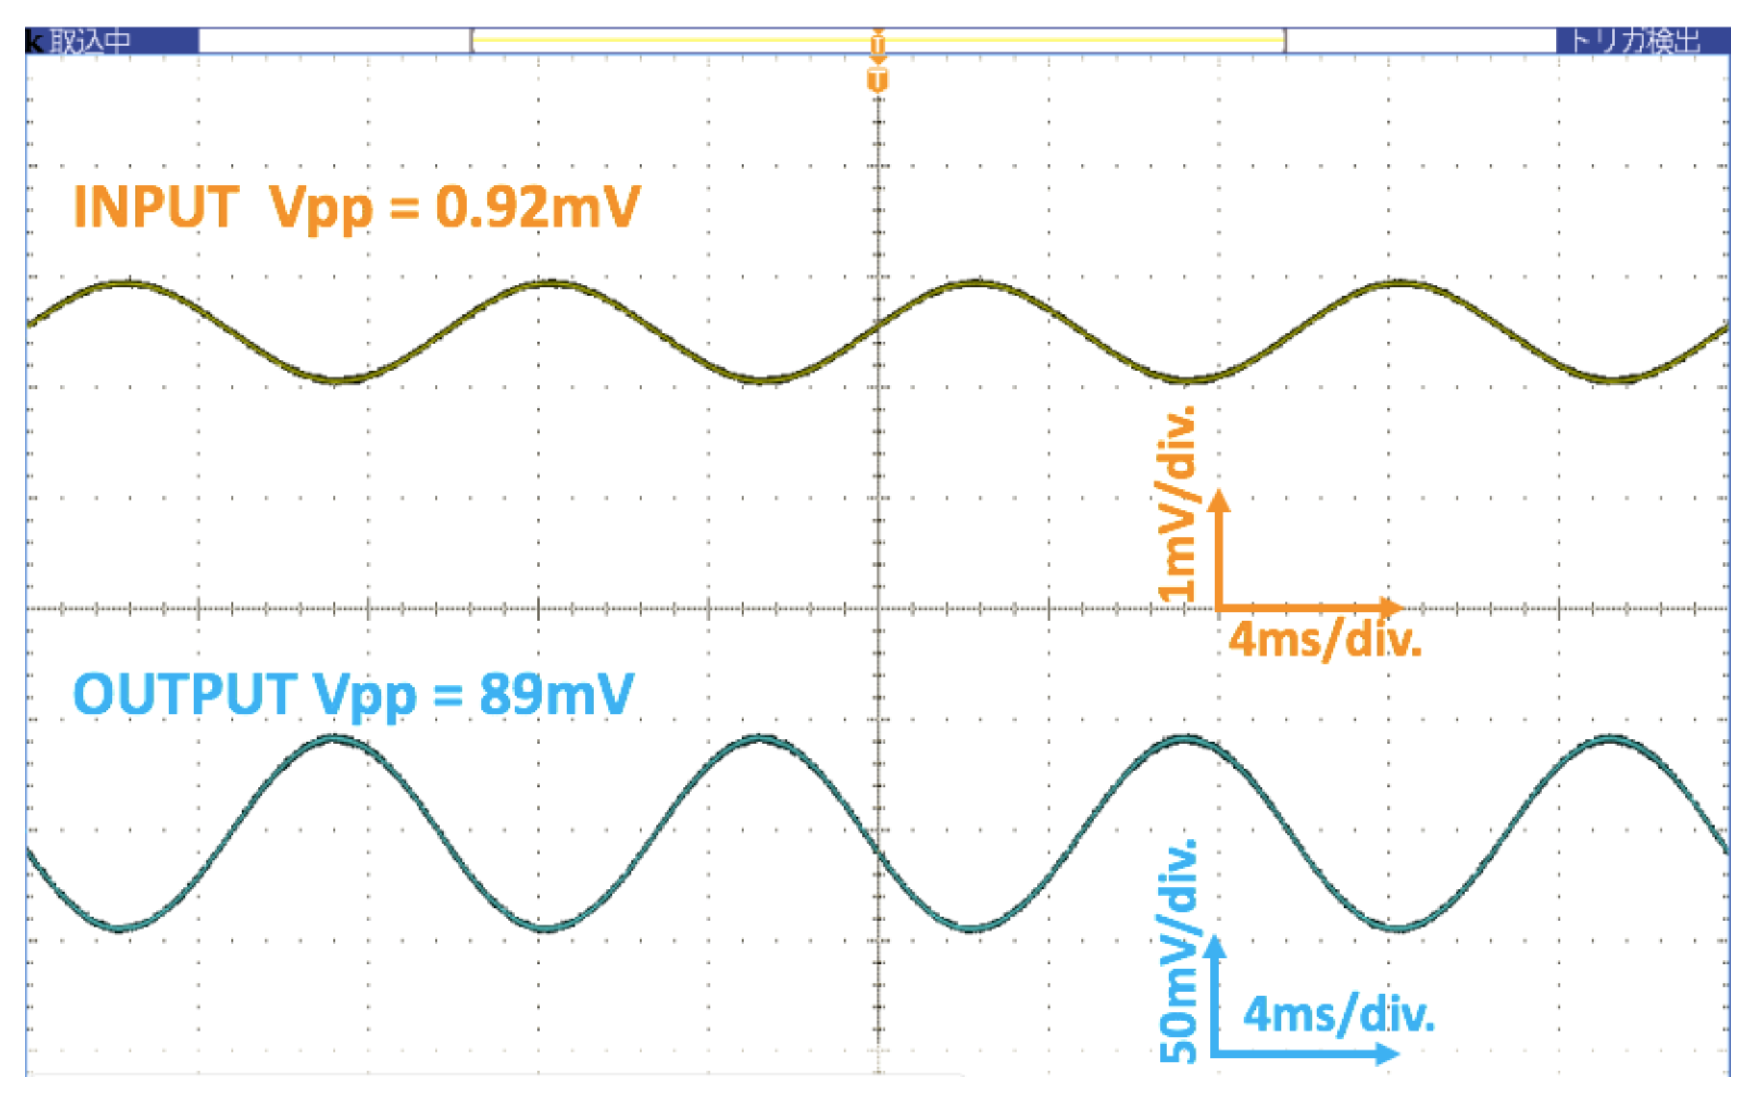
\includegraphics[width=12.0cm]{./Chapter/Chapter4/Picture/SOISTJ4wSTJ_InOut_100Hz.eps}
					\caption{Nb/Al-STJ検出器と組み合わせた回路でのSOI-STJ4を用いたsin波増幅試験\ 入出力波形($f_{\mathrm{input}}=100\mathrm{Hz}$)}
					\label{fig:SOISTJ4wSTJ_InOut_100Hz}
				\end{center}
			\end{figure}
			\begin{figure}[htbp]
				\begin{center}
					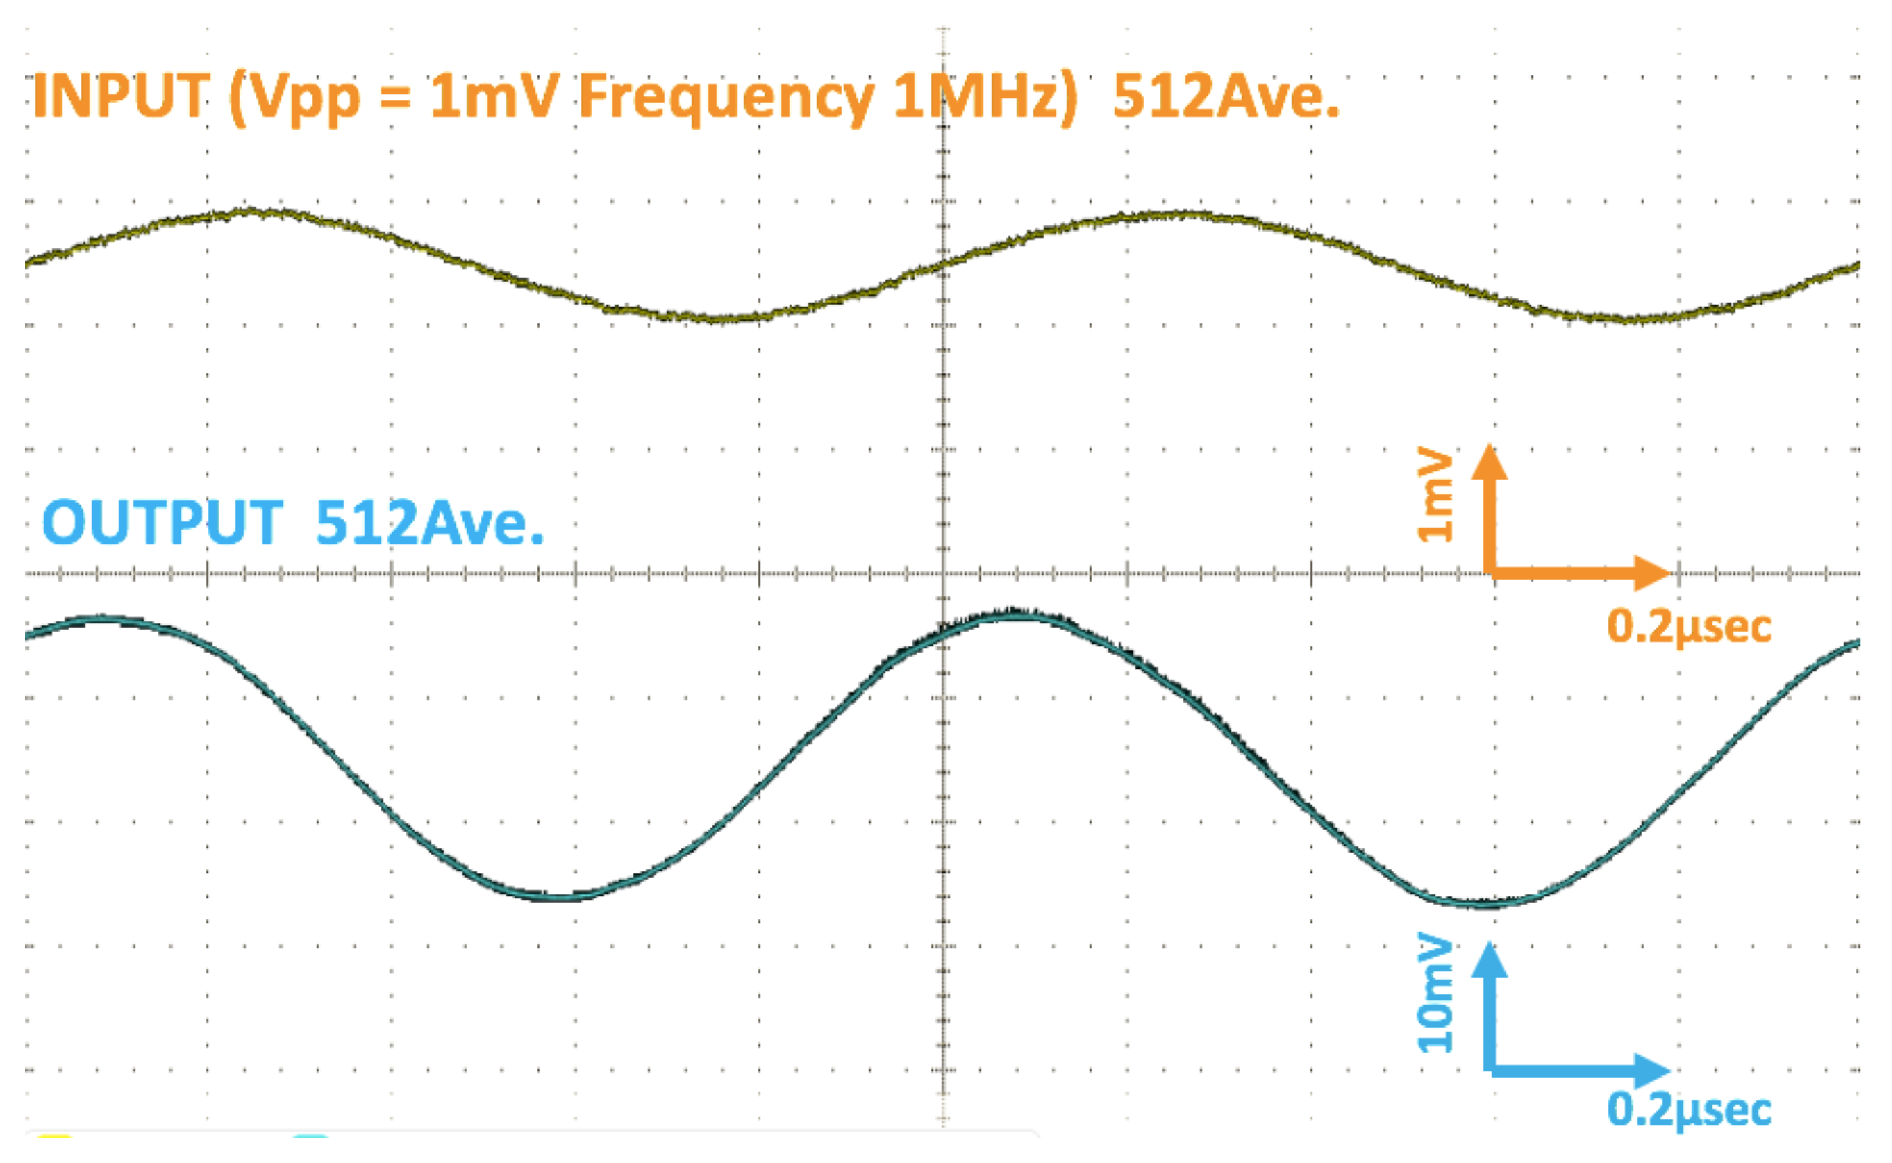
\includegraphics[width=12.0cm]{./Chapter/Chapter4/Picture/SOISTJ4wSTJ_InOut_1MHz.eps}
					\caption{Nb/Al-STJ検出器と組み合わせた回路でのSOI-STJ4を用いたsin波増幅試験\ 入出力波形($f_{\mathrm{input}}=1\mathrm{MHz}$)}
					\label{fig:SOISTJ4wSTJ_InOut_1MHz}
				\end{center}
			\end{figure}
			\begin{figure}[htbp]
				\begin{center}
					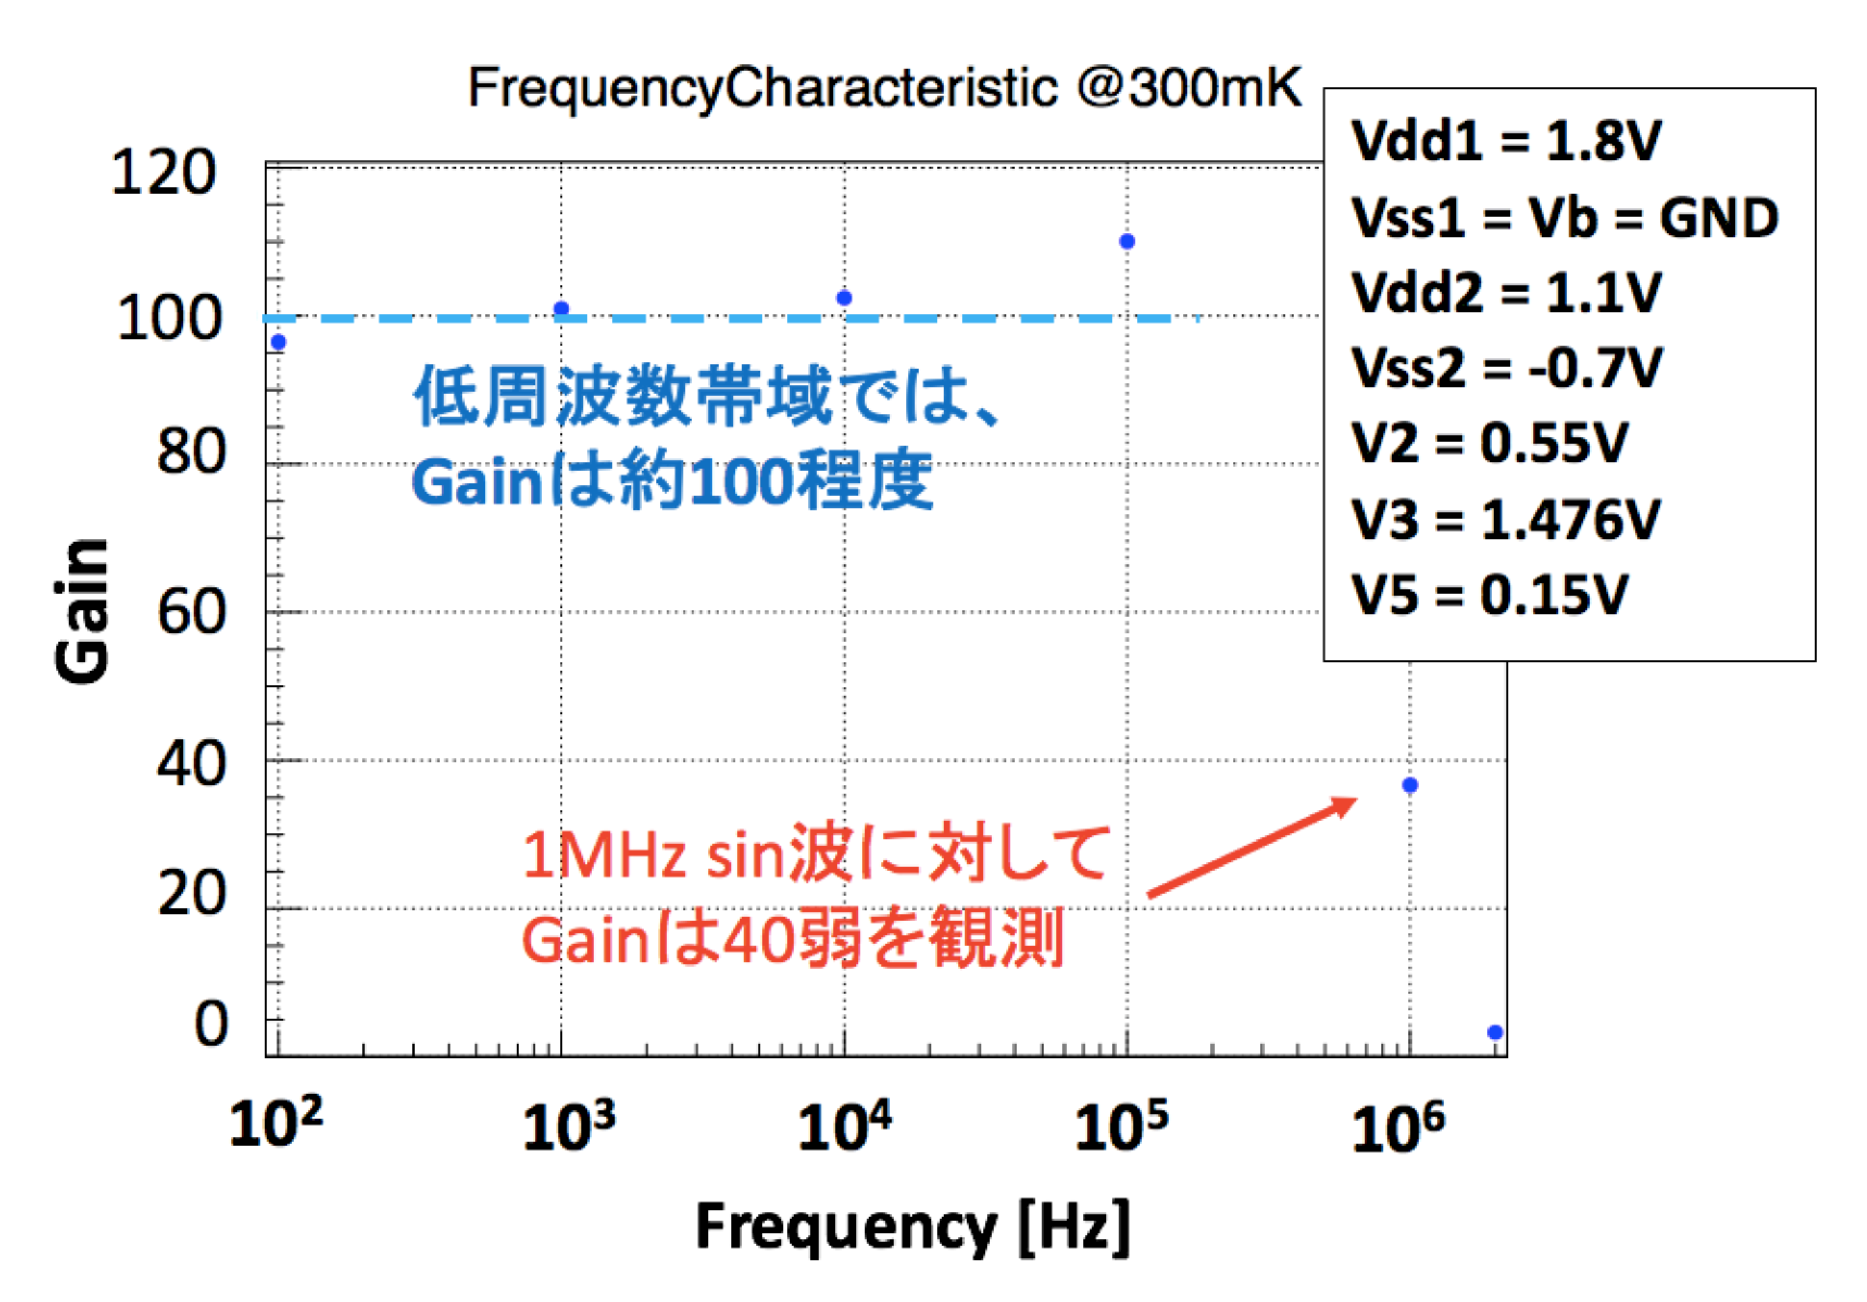
\includegraphics[width=12.0cm]{./Chapter/Chapter4/Picture/SOISTJ4wSTJ_frequency.eps}
					\caption{Nb/Al-STJ検出器と組み合わせた回路でのSOI-STJ4を用いたsin波増幅試験\ 利得の周波数依存性}
					\label{fig:SOISTJ4wSTJ_frequency}
				\end{center}
			\end{figure}
			\clearpage
			
	\section{SOI増幅器とNb/Al-STJ検出器を組み合わせた回路での \newline Nb/Al-STJ検出器の電流電圧特性の測定}
		\begin{figure}[htbp]
			\begin{center}
				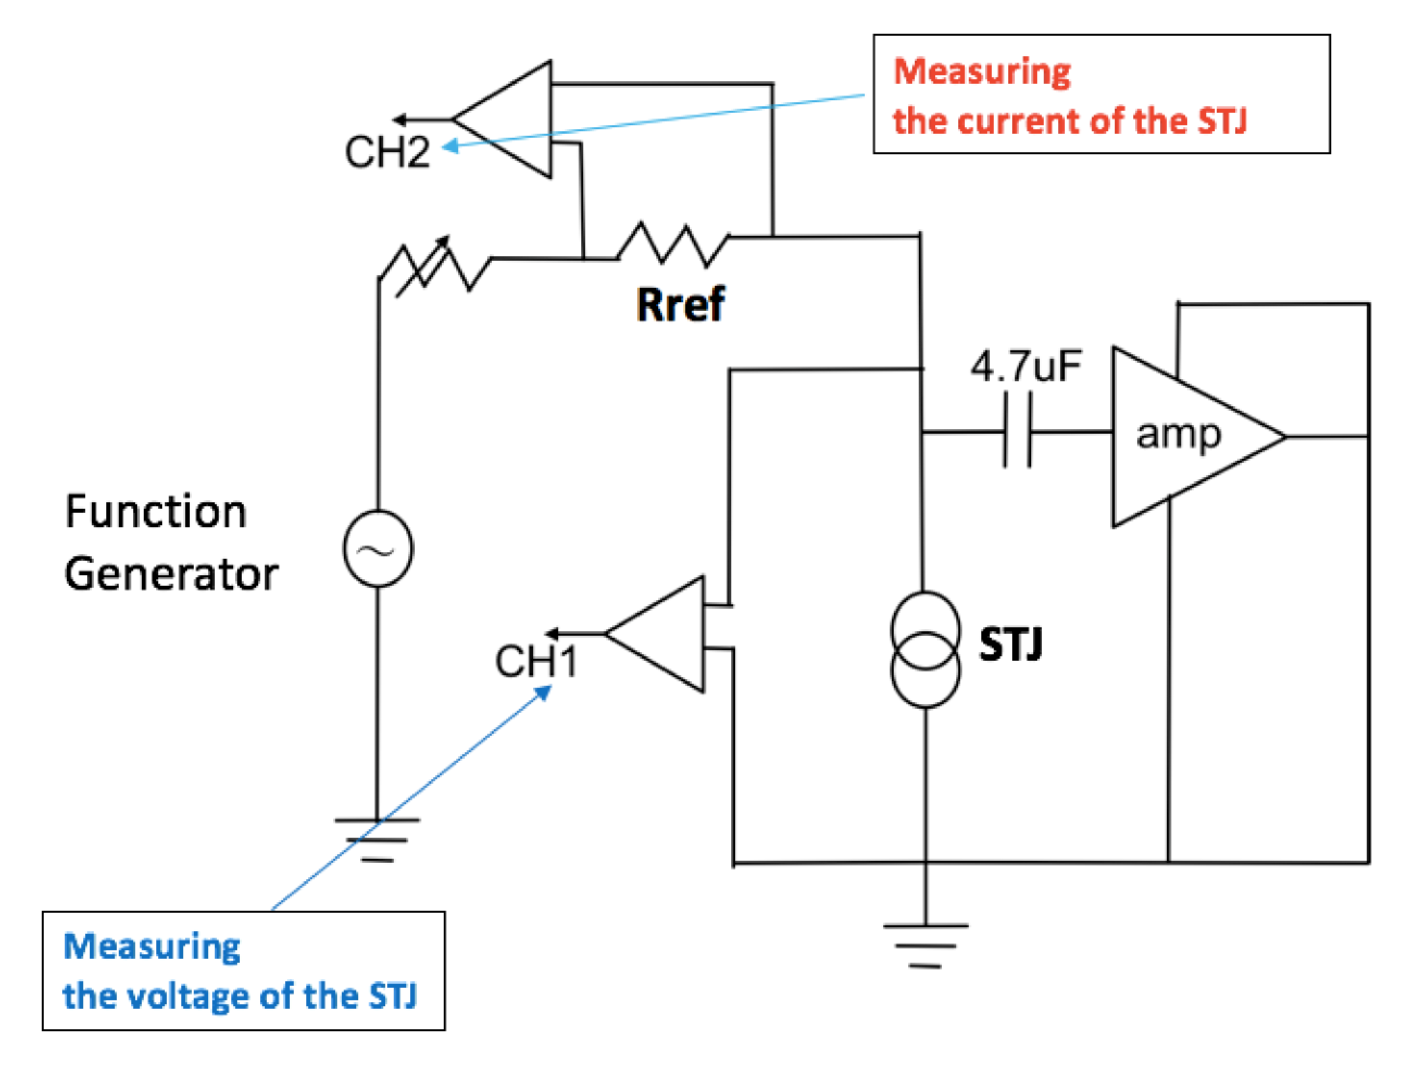
\includegraphics[width=8.0cm]{./Chapter/Chapter4/Picture/NbAlSTJwSOI_IV_circuit.eps}
				\caption{SOI-STJ4と組み合わせた回路でのNb/Al-STJ検出器の電流電圧特性\ 回路図}
				\label{fig:NbAlSTJwSOI_IV_circuit}
			\end{center}
		\end{figure}
		前節ではSOI-STJ4の性能評価について述べた。
		本節では、SOI-STJ4と組み合わせた回路上でNb/Al-STJ検出器の電流電圧特性について述べる。
		この測定の結果を用いて、SOI-STJ4を用いたNb/Al-STJ検出器信号増幅試験において、STJ検出器に流す定電流値を決める。
		
		本測定回路図を図\ref{fig:NbAlSTJwSOI_IV_circuit}に示す。
		Nb/Al-STJ検出器の電流電圧特性を基本的には4端子法で測定する。
		図\ref{fig:NbAlSTJwSOI_IV_circuit}中のCH1でSTJ検出器の両端電圧を読み出す。
		一方、図\ref{fig:NbAlSTJwSOI_IV_circuit}中のCH2では基準抵抗$\mathrm{R_{ref}}$間の両端の電圧を読み出すことで、Ohmの法則を用いてSTJ検出器に流れる電流値を計算する。
		
		注意すべきことは、SOI-STJ4とNb/Al-STJ検出器は$4.7\mathrm{\mu F}$のキャパシタンスでAC的に区切っている。
		しかし、SOI-STJ4が動作してしまうとSTJ検出器の電流電圧特性が変化して観測されてしまうので、SOI-STJ4の全ての端子をGNDに落として動作しないようにした。
		
		電流電圧特性の測定結果を図\ref{fig:NbAlSTJwSOI_IV_chara}に示す。
		本測定では0V付近でヒステリシス構造を持ち、図\ref{fig:STJ_IV}のような一般的なSTJ検出器の電流電圧特性と異なる構造を持つ。
		この原因として、我々が使う$\mathrm{^{3}He}$減圧冷凍機に搭載されている超電導コイルの不調でジョセフソン電流を抑制しきれなかったのが原因だと考えている。
		本節では超電導コイルが不調のままSOI-STJ4を用いたSTJ検出器信号増幅試験を行い、超電導コイル修理後にジョセフソン電流を十分抑制しきった状態で再試験を行う。
		\clearpage
		\begin{figure}[htbp]
			\begin{center}
				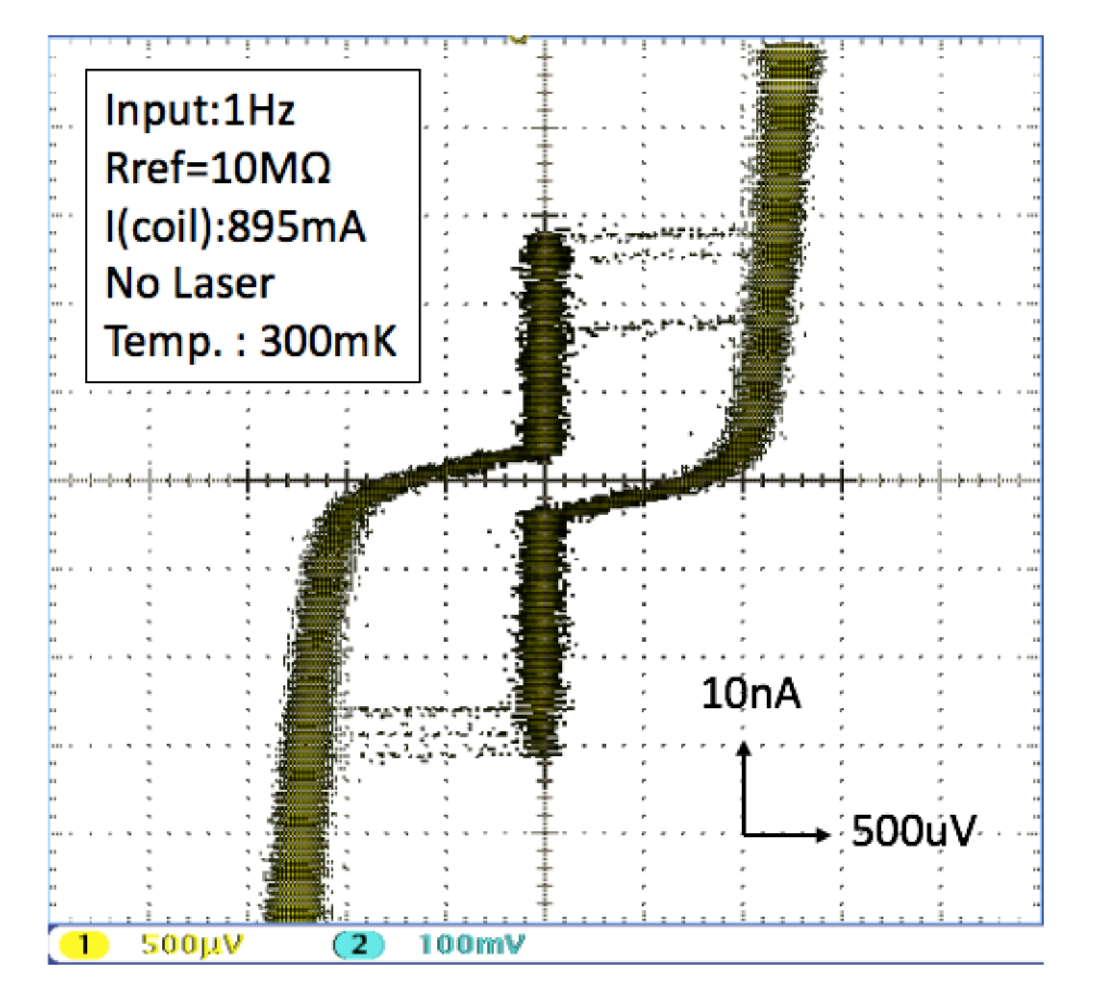
\includegraphics[width=10.0cm]{./Chapter/Chapter4/Picture/NbAlSTJwSOI_IV_chara.eps}
				\caption{SOI-STJ4と組み合わせた回路でのNb/Al-STJ検出器の電流電圧特性}
				\label{fig:NbAlSTJwSOI_IV_chara}
			\end{center}
		\end{figure}
		\begin{figure}[htbp]
			\begin{center}
				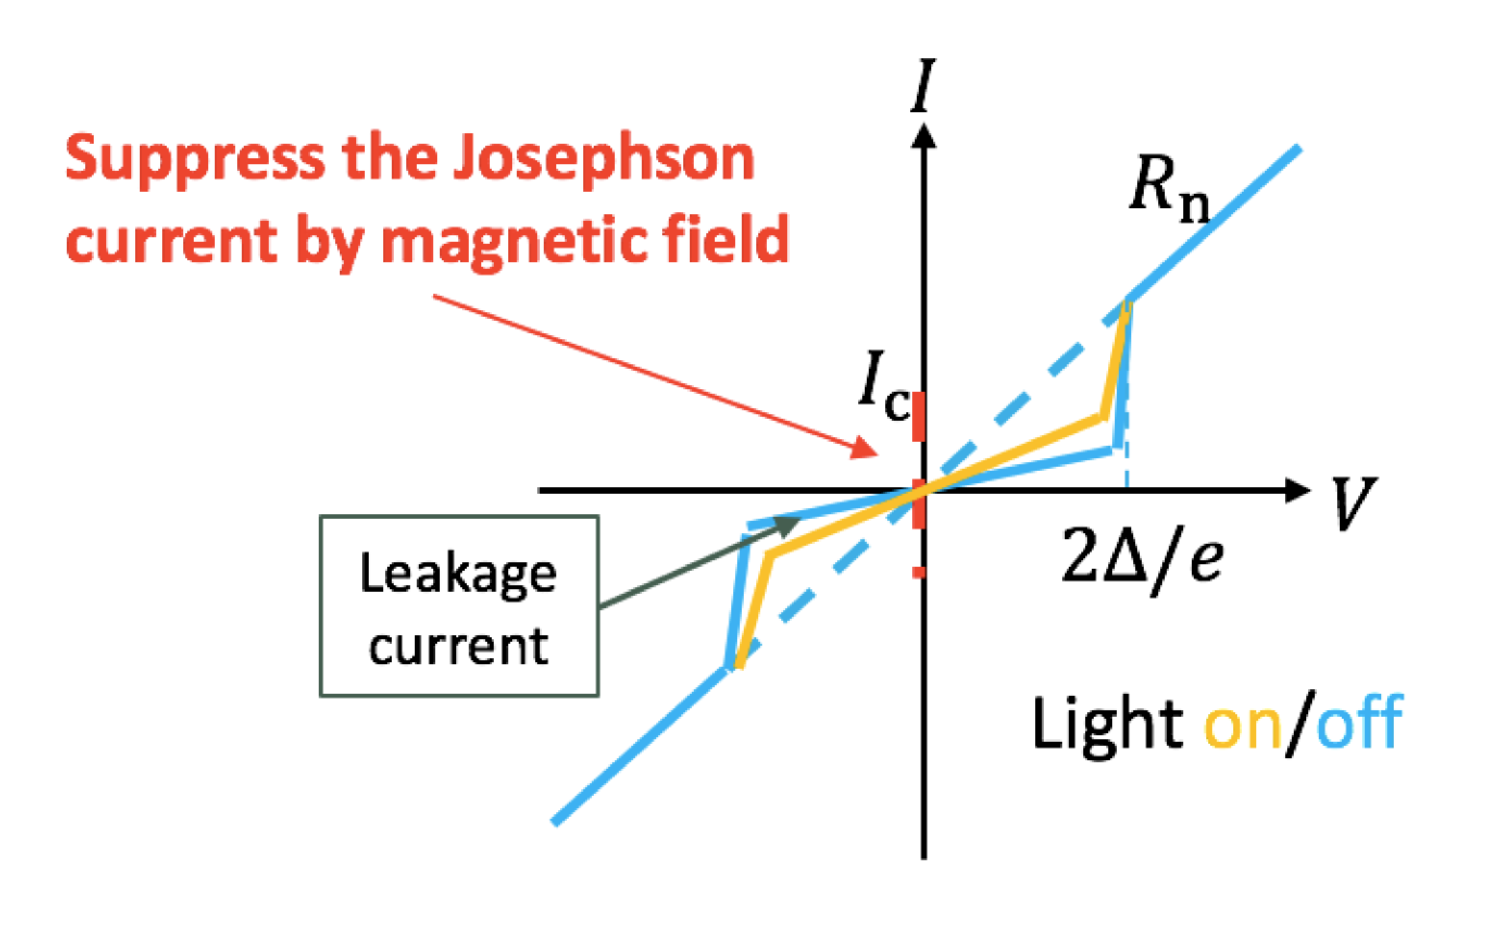
\includegraphics[width=10.0cm]{./Chapter/Chapter4/Picture/STJ_IV.eps}
				\caption{一般的なSTJ検出器の電流電圧特性}
				\label{fig:STJ_IV}
			\end{center}
		\end{figure}
		\clearpage
		
		次に、図\ref{fig:NbAlSTJwSOI_IV_circuit}の回路のまま、STJ検出器に可視光レーザーを照射したときに電流電圧特性がどのように変化するかを評価した。
		照射に用いた可視光レーザー(HAMAMATSU PICOSECOND LIGHT PULSER)の性能については表\ref{tab:lazer}に記した。
		\begin{table}[htb]
			\begin{center}
				\begin{tabular}{| l | l |} \hline
					レーザー & HAMAMATSU PICOSECOND LIGHT PULSER \\ \hline
					波長 & $465 \mathrm{nm}$ \\ \hline
					パルス幅 & $59$ps \\ \hline
					最大ピーク出力 & $149$mW \\ \hline \hline
					備考 & 1Hz〜100MHzの周波数で連続的に照射可能 \\ \hline
				\end{tabular}
				\caption{レーザーコントローラーの性能表}
				\label{tab:lazer}
			\end{center}
		\end{table}
		
		レーザー周波数を変化させたときのSTJ検出器の電流電圧特性を図\ref{fig:NbAlSTJwSOI_IV_chara_lazer}に示した。
		$-30 \mathrm{\mu A}$〜$30 \mathrm{nA}$でヒステリシス構造がある。
		本来この領域でSTJ検出器を動作させるが、このヒステリシス構造のため光応答試験においてこの領域は使えない。
		$30\mathrm{\mu A}$〜$50\mathrm{nA}$の領域において、レーザー照射「あり」の場合と「なし」の場合で0.1mV程度の応答が見える。
		SOI増幅器を用いたSTJ検出器信号増幅試験では、この領域でSTJ検出器を動作させる。
		\begin{figure}[htbp]
			\begin{center}
				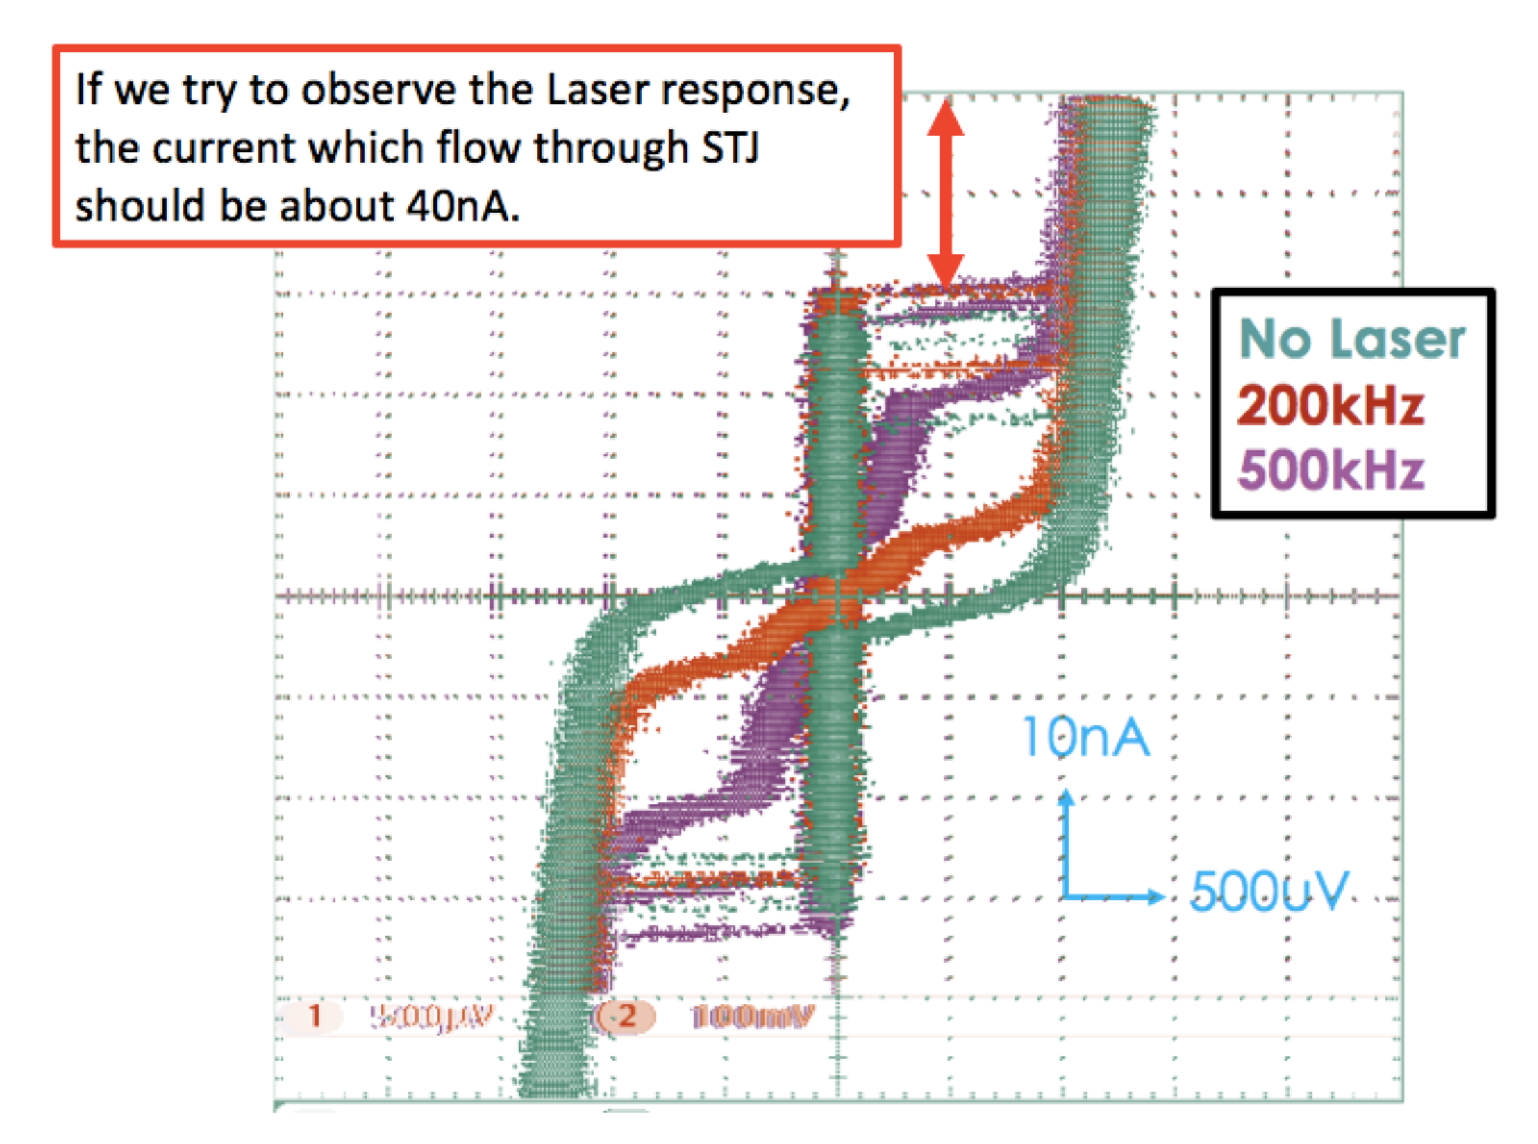
\includegraphics[width=10.0cm]{./Chapter/Chapter4/Picture/NbAlSTJwSOI_IV_chara_lazer.eps}
				\caption{SOI-STJ4と組み合わせた回路でのNb/Al-STJ検出器の電流電圧特性\ レーザーを照射しながら測定した}
				\label{fig:NbAlSTJwSOI_IV_chara_lazer}
			\end{center}
		\end{figure}
		
		\clearpage
	\section{SOI増幅器を用いたSTJ検出器信号増幅試験}
		\begin{figure}[htbp]
			\begin{center}
				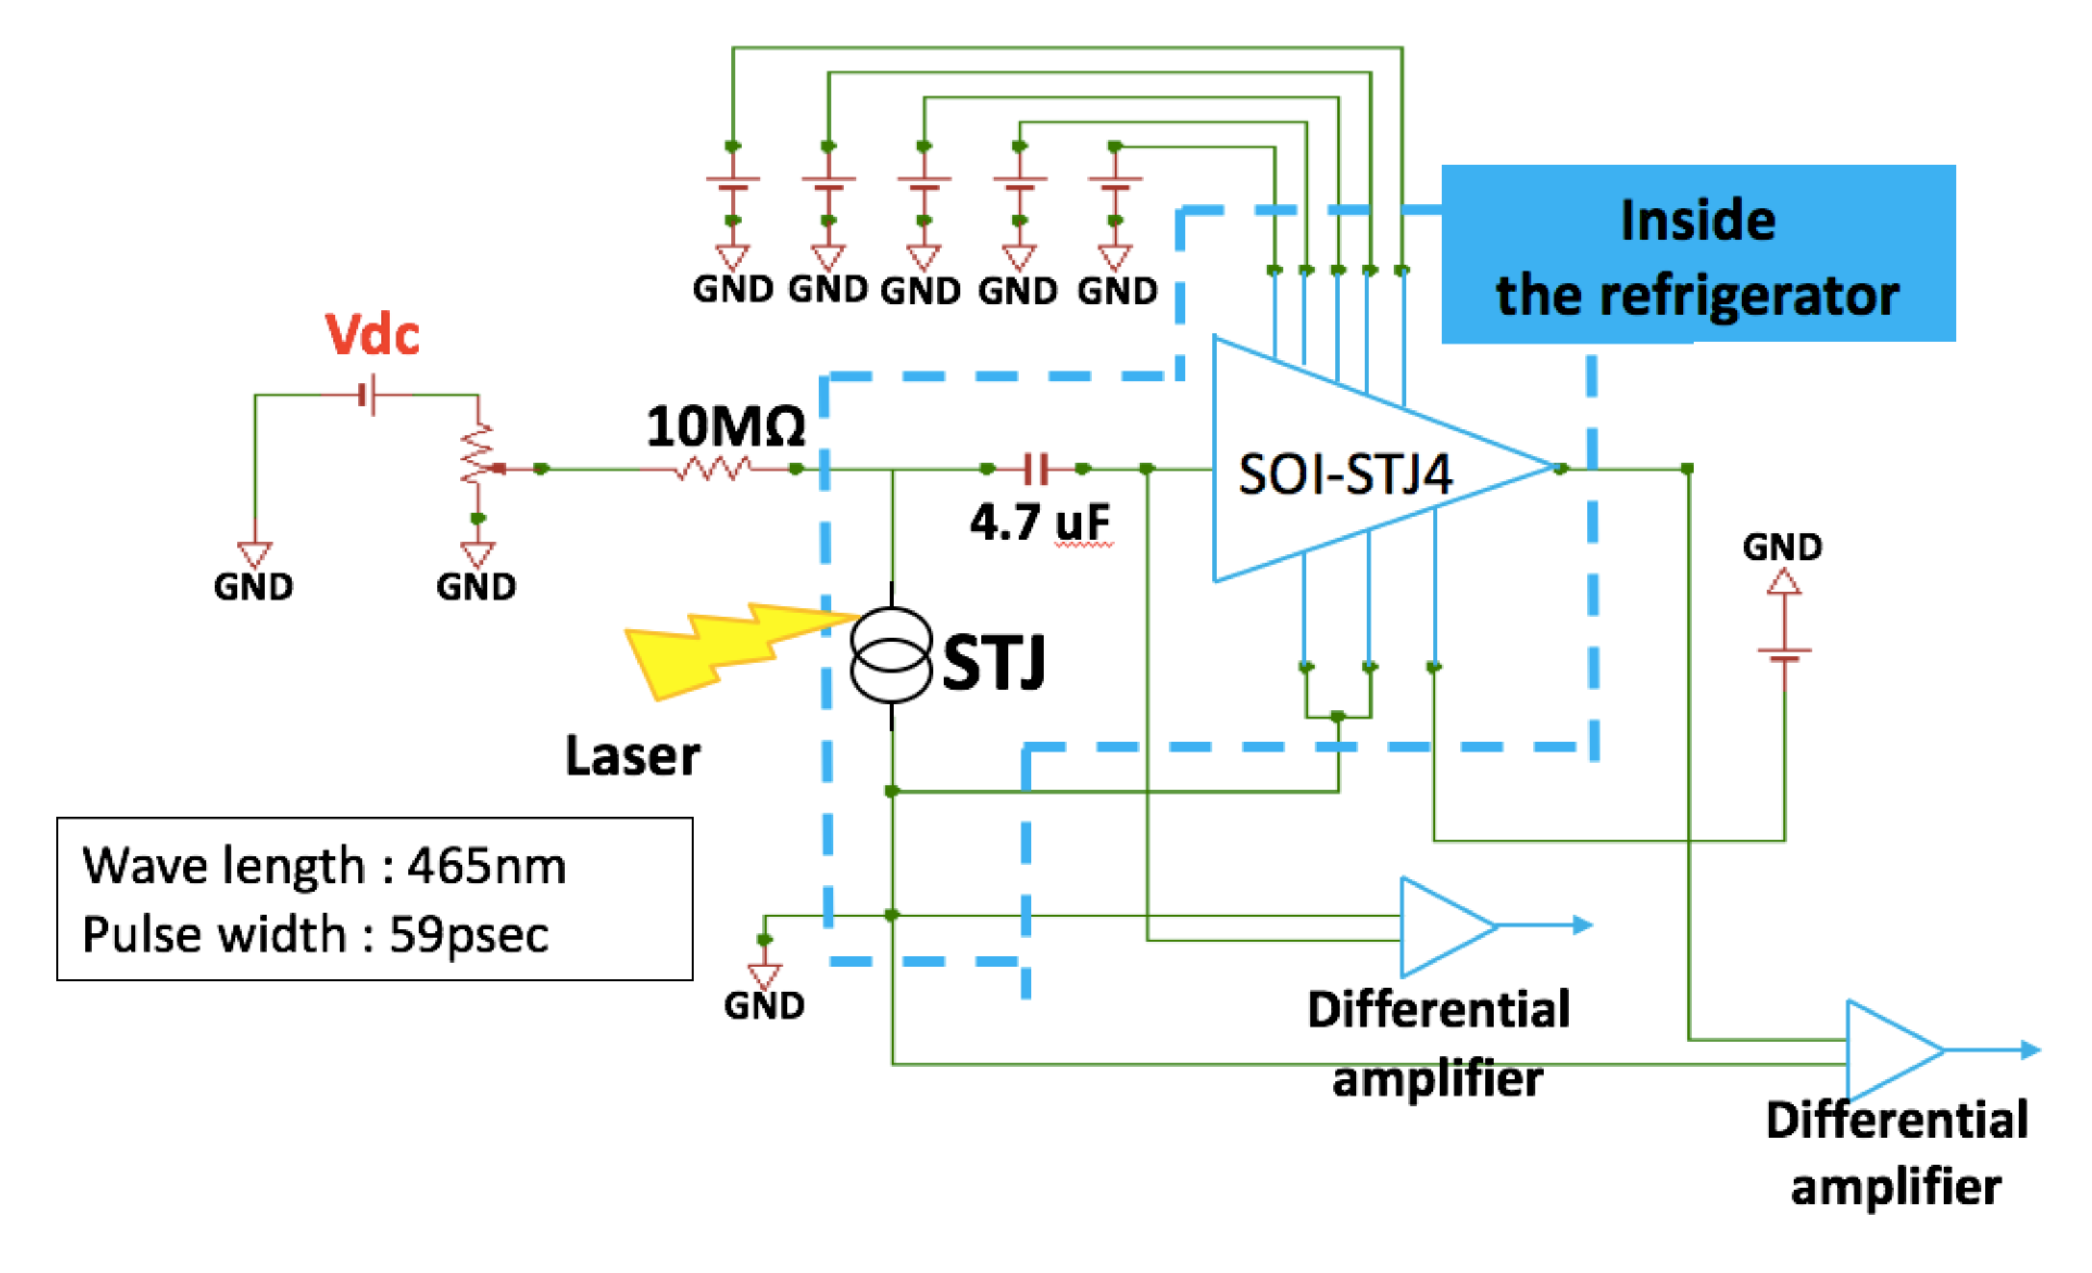
\includegraphics[width=10.0cm]{./Chapter/Chapter4/Picture/STJamp_circuit.eps}
				\caption{SOI-STJ4を用いたSTJ検出器信号増幅試験\ 回路図}
				\label{fig:STJamp_circuit}
			\end{center}
		\end{figure}
		本節ではSOI-STJ4を用いたNb/Al-STJ検出器信号増幅試験について述べる。
		増幅試験での回路図を図\ref{fig:STJamp_circuit}に示す。
		直流電源$\mathrm{V_{dc}}$と基準抵抗$10\mathrm{M\Omega}$をSTJ検出器に対して直列に接続する。
		Dynamic resistance領域でのSTJ検出器の抵抗は約$1\mathrm{M\Omega}$程度である。
		前節で述べたようにSTJ検出器には約$40\mathrm{nA}$程度の定電流を流しながら動作させたいので、直流電源$\mathrm{V_{dc}}$には0.4V程度印加する。
		もしSTJ検出器信号の波高が小さすぎる場合はこの直流電源を微調整する。
		レーザーは前節で述べた可視光レーザーを使用した。

		レーザー照射することでSTJ検出器の両端電圧が変化し、その信号をSOI-STJ4へ伝送することを考えている。
		SOI-STJ4の入力インピーダンスは約$200\mathrm{k\Omega}$程度であり、さらに1MHz帯域の信号に対して$4.7\mathrm{\mu F}$のキャパシタンスのインピーダンスは非常に小さい。
		このことから、STJ検出器信号はほぼSOI-STJ4側へ伝送される。
		
		本測定で我々は以下の2点について検証する。
		\begin{itemize}
			\item STJ検出器信号がSOI-STJ4へ伝送されるか
			\item 伝送されたSTJ検出器信号がSOI-STJ4を用いて増幅できるか
		\end{itemize}
		
		SOI-STJ4の入出力波形は差動増幅器とオシロスコープを用いて読み出された。
		オシロスコープの設定は、前節と同様
		\begin{itemize}
			\item 入力インピーダンス\ $1\mathrm{M \Omega}$
			\item AC結合
			\item 512回平均
		\end{itemize}
		である。
		
		\clearpage
		
		\subsection{測定結果}
			\begin{figure}[htbp]
				\begin{center}
					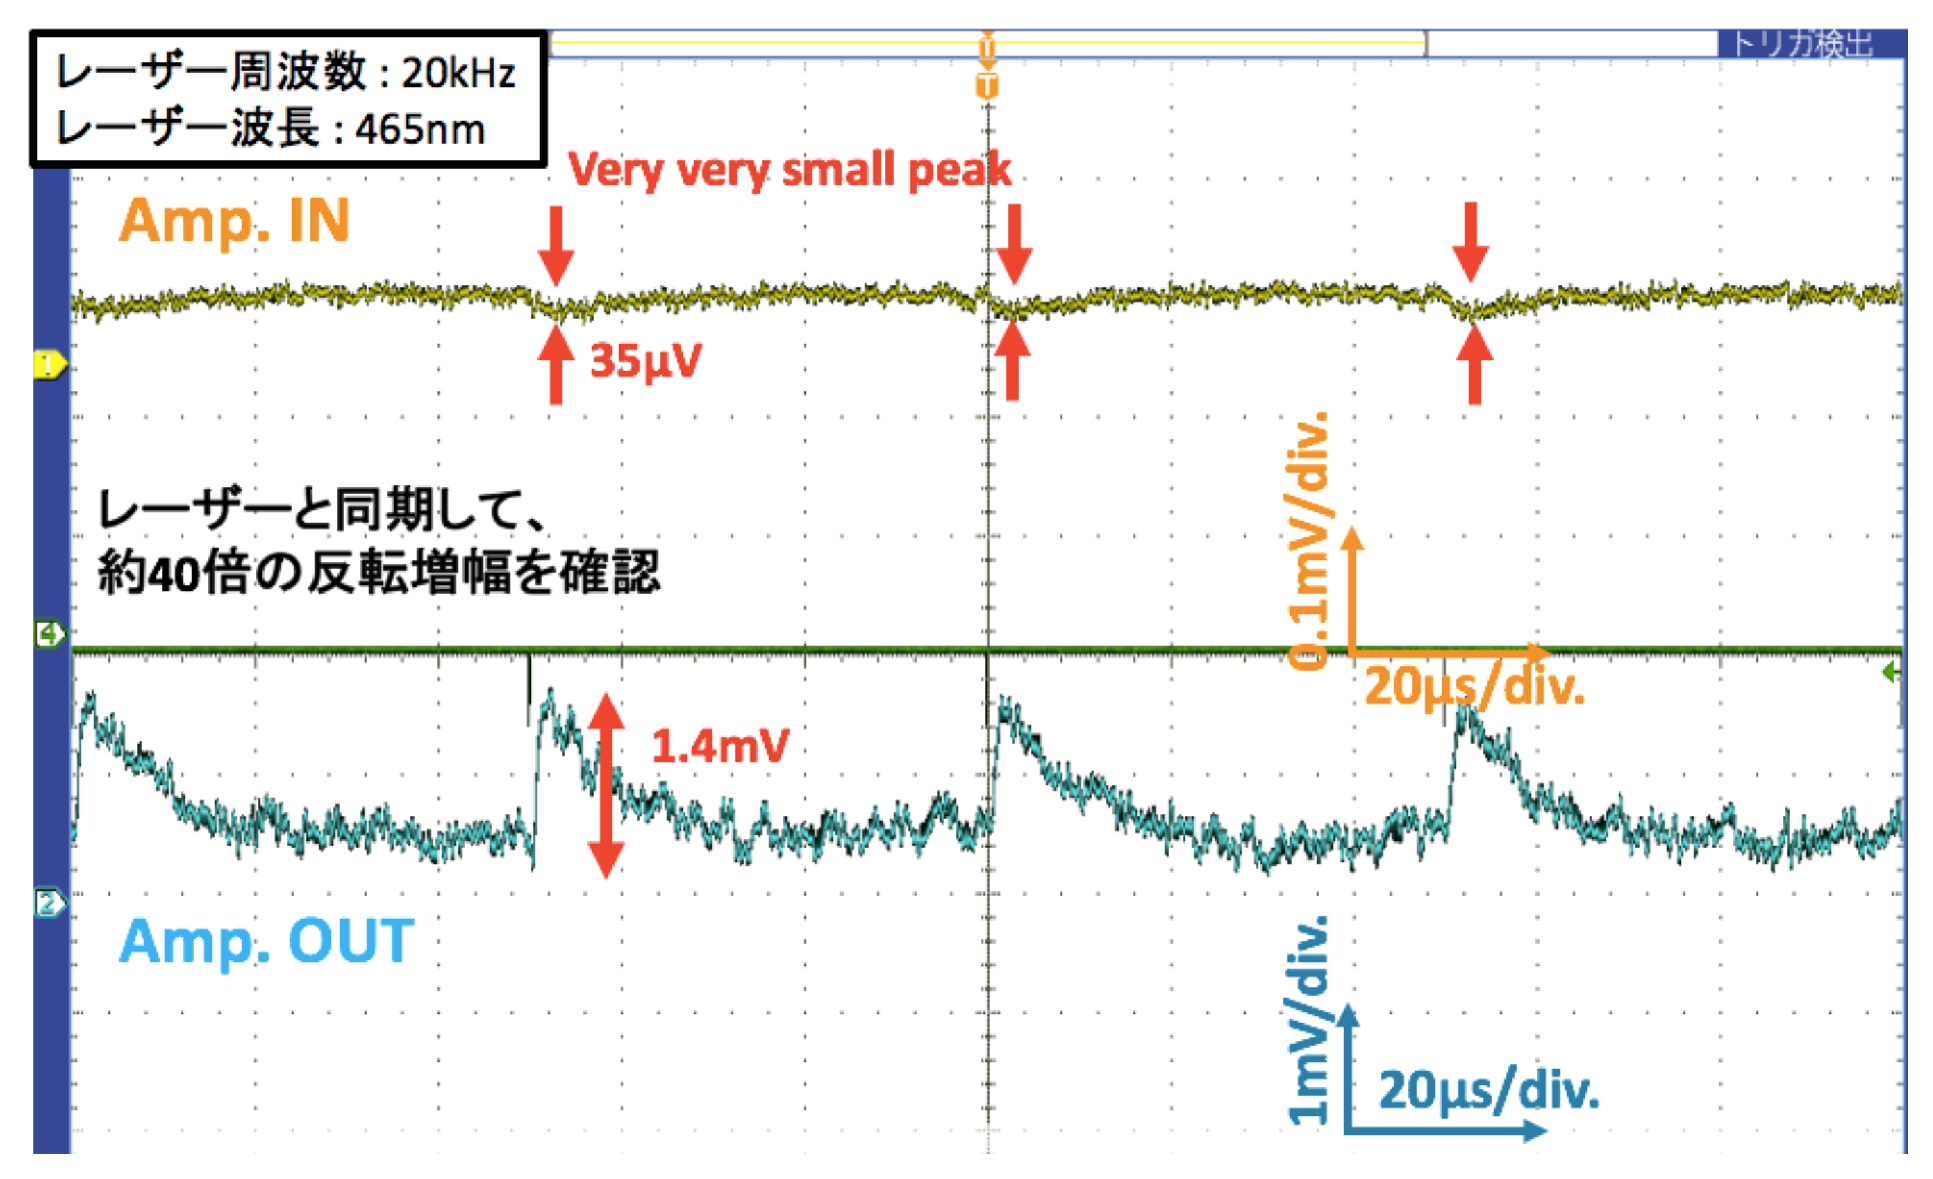
\includegraphics[width=10.0cm]{./Chapter/Chapter4/Picture/STJamp_lazer20k_raw.eps}
					\caption{SOI-STJ4を用いたSTJ検出器信号増幅試験(レーザー周波数$f_{\mathrm{lazer}=20\mathrm{kHz}}$\ 直流電源$V_{\mathrm{dc}}=0.43\mathrm{V}$)}
					\label{fig:STJamp_lazer20k_raw}
				\end{center}
			\end{figure}
		
			\begin{figure}[htbp]
				\begin{center}
					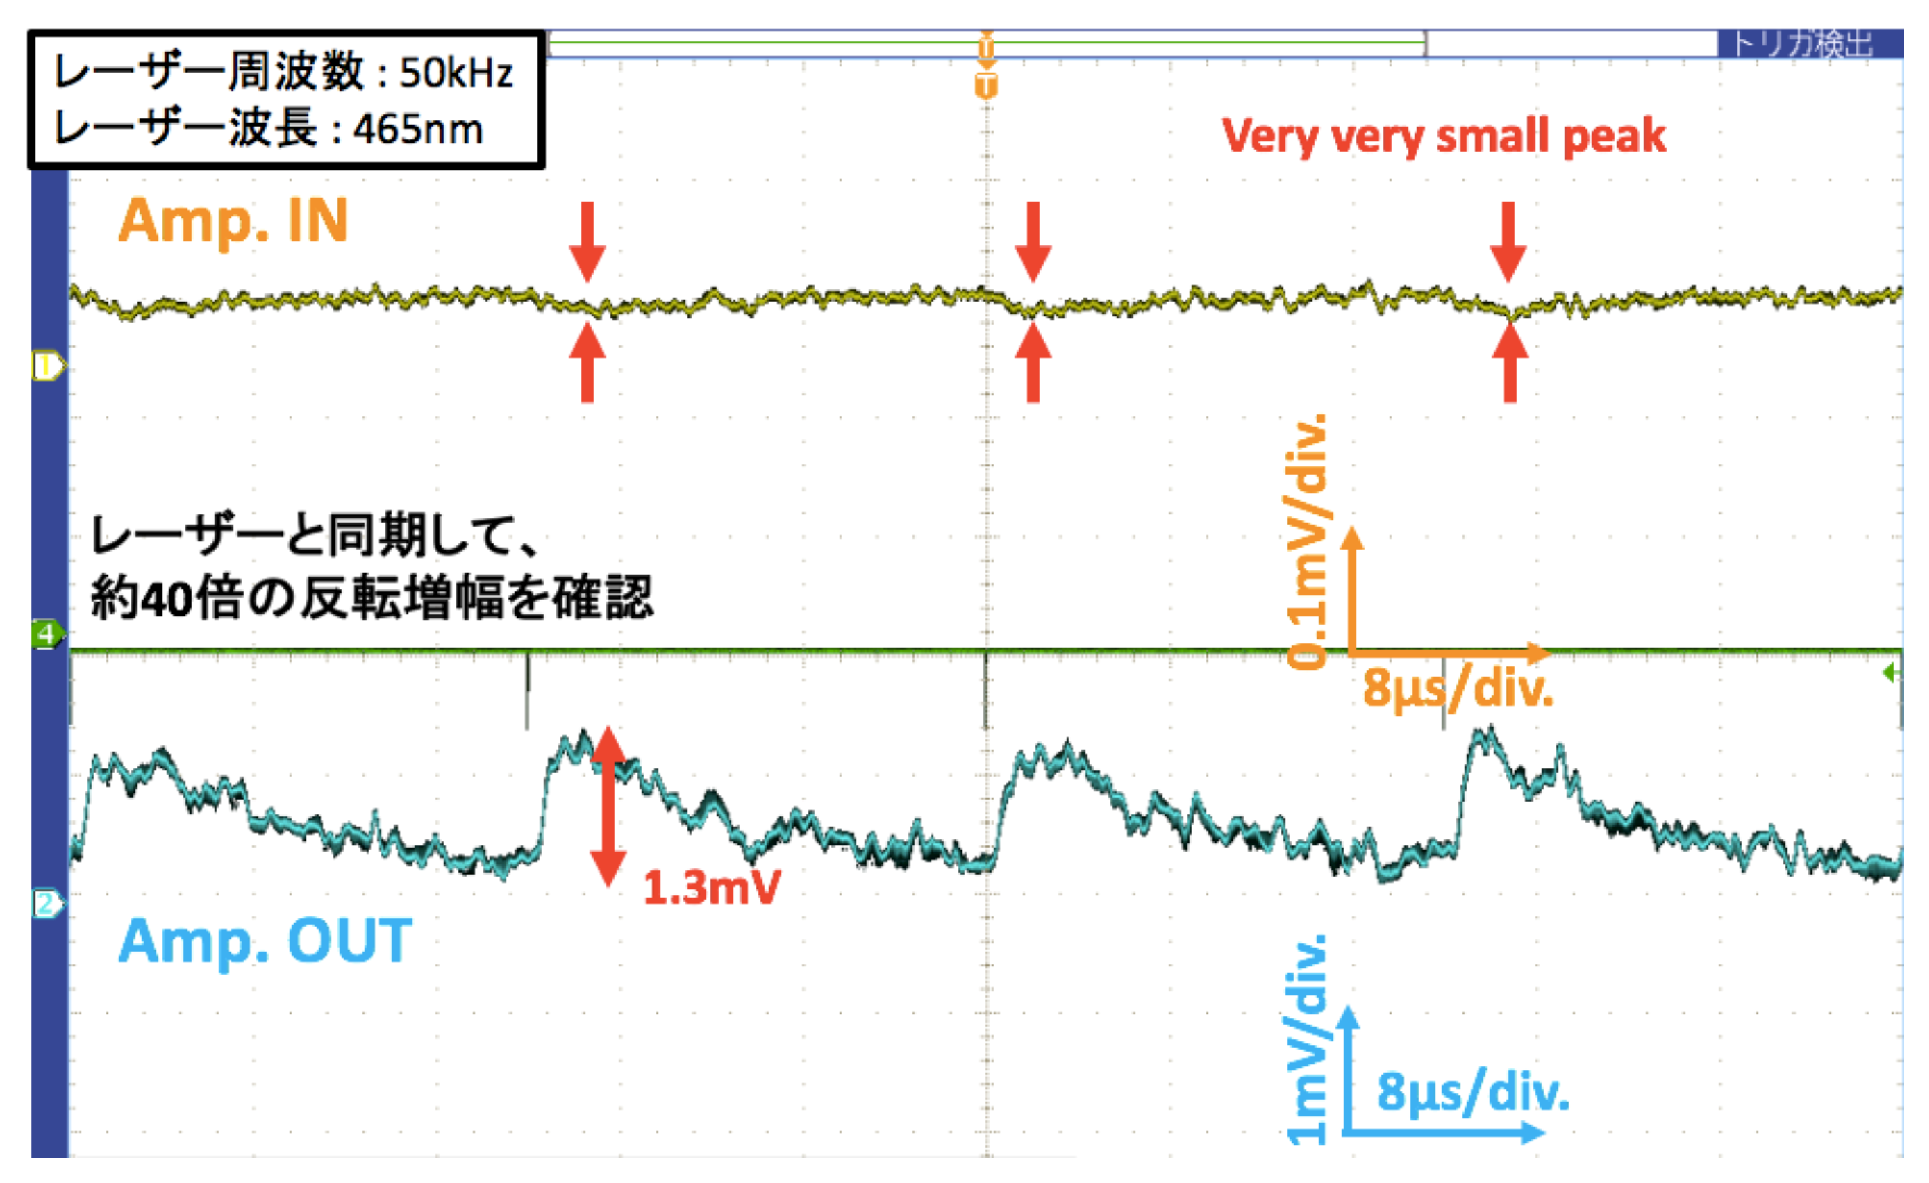
\includegraphics[width=10.0cm]{./Chapter/Chapter4/Picture/STJamp_lazer50k_raw.eps}
					\caption{SOI-STJ4を用いたSTJ検出器信号増幅試験(レーザー周波数$f_{\mathrm{lazer}=50\mathrm{kHz}}$\ 直流電源$V_{\mathrm{dc}}=0.43\mathrm{V}$)}
					\label{fig:STJamp_lazer50k_raw}
				\end{center}
			\end{figure}
			レーザー周波数を20kHzにした場合のSOI-STJ4への入力と出力の結果を図\ref{fig:STJamp_lazer20k_raw}に示した。
			同様に50kHzにした場合の結果を図\ref{fig:STJamp_lazer50k_raw}に示した。
			各図の黄線はSOI-STJ4への入力波形を示し、青線はSOI-STJ4の出力波形を示す。
			
			各図入力波形を見るとレーザーと同期して非常に小さなスパイクを観測できた。
			同様に出力波形を見るとレーザーと同期して正のピークを観測した。
			
			図\ref{fig:STJamp_lazer20k_raw_kakudai}と図\ref{fig:STJamp_lazer50k_raw_kakudai}入力波形の波高がかなり小さいので拡大した図である。
			各図の青線はSOI-STJ4への入力波形、橙線はSOI-STJ4の出力波形を示す。
			これらを見るとSOI-STJ4への入力波形は負のピークを持つことがわかる。
			各レーザー周波数ごとに入出力の波高を表\ref{tab:STJamp_vpp}に示した。
			\begin{table}[htb]
				\begin{center}
					\begin{tabular}{| l || l | l |} \hline
						レーザー周波数 & 入力波高 & 出力波高 \\ \hline \hline
						$20\mathrm{kHz}$ & $35 \mathrm{\mu V}$ & $1.4\mathrm{mV}$ \\ \hline
						$50\mathrm{kHz}$ & $33 \mathrm{\mu V}$ & $1.3\mathrm{mV}$ \\ \hline
					\end{tabular}
					\caption{レーザー周波数ごとの入出力波高}
					\label{tab:STJamp_vpp}
				\end{center}
			\end{table}
			
			SOI-STJ4への入力波形が、レーザーと同期して負にピークを持っている。
			レーザーを照射しながらSTJ検出器の電流電圧特性を測定した際、本測定で動作させる領域においてIVカーブが電圧が負の方向にシフトしていた。
			これらから、STJ検出器信号がSOI-STJ4に伝送されていたことがわかる。
			
			一方、SOI-STJ4の出力波形は入力波形とは逆に正のピークを持っている。
			SOI-STJ4のsin波増幅試験の結果の通り、SOI-STJ4回路には増幅段にソース接地増幅回路が入っているので入力に対して反転して増幅する。
			これらから、SOI-STJ4へ伝送されたSTJ検出器信号がSOI-STJ4で増幅されたことが実証された。
			
			FD-SOI-MOSFETを用いた前置増幅器が極低温環境下(300mK環境下)で信号読み出し可能であることから、我々が関わる素粒子実験分野に留まらず、低温読み出しを行う他分野への応用も期待される。
			
			今後としては、本実験でのSOI-STJ4に伝送された信号は何光子相当であったかなど、より定量的な解析を行う必要がある。
			\begin{figure}[htbp]
				\begin{center}
					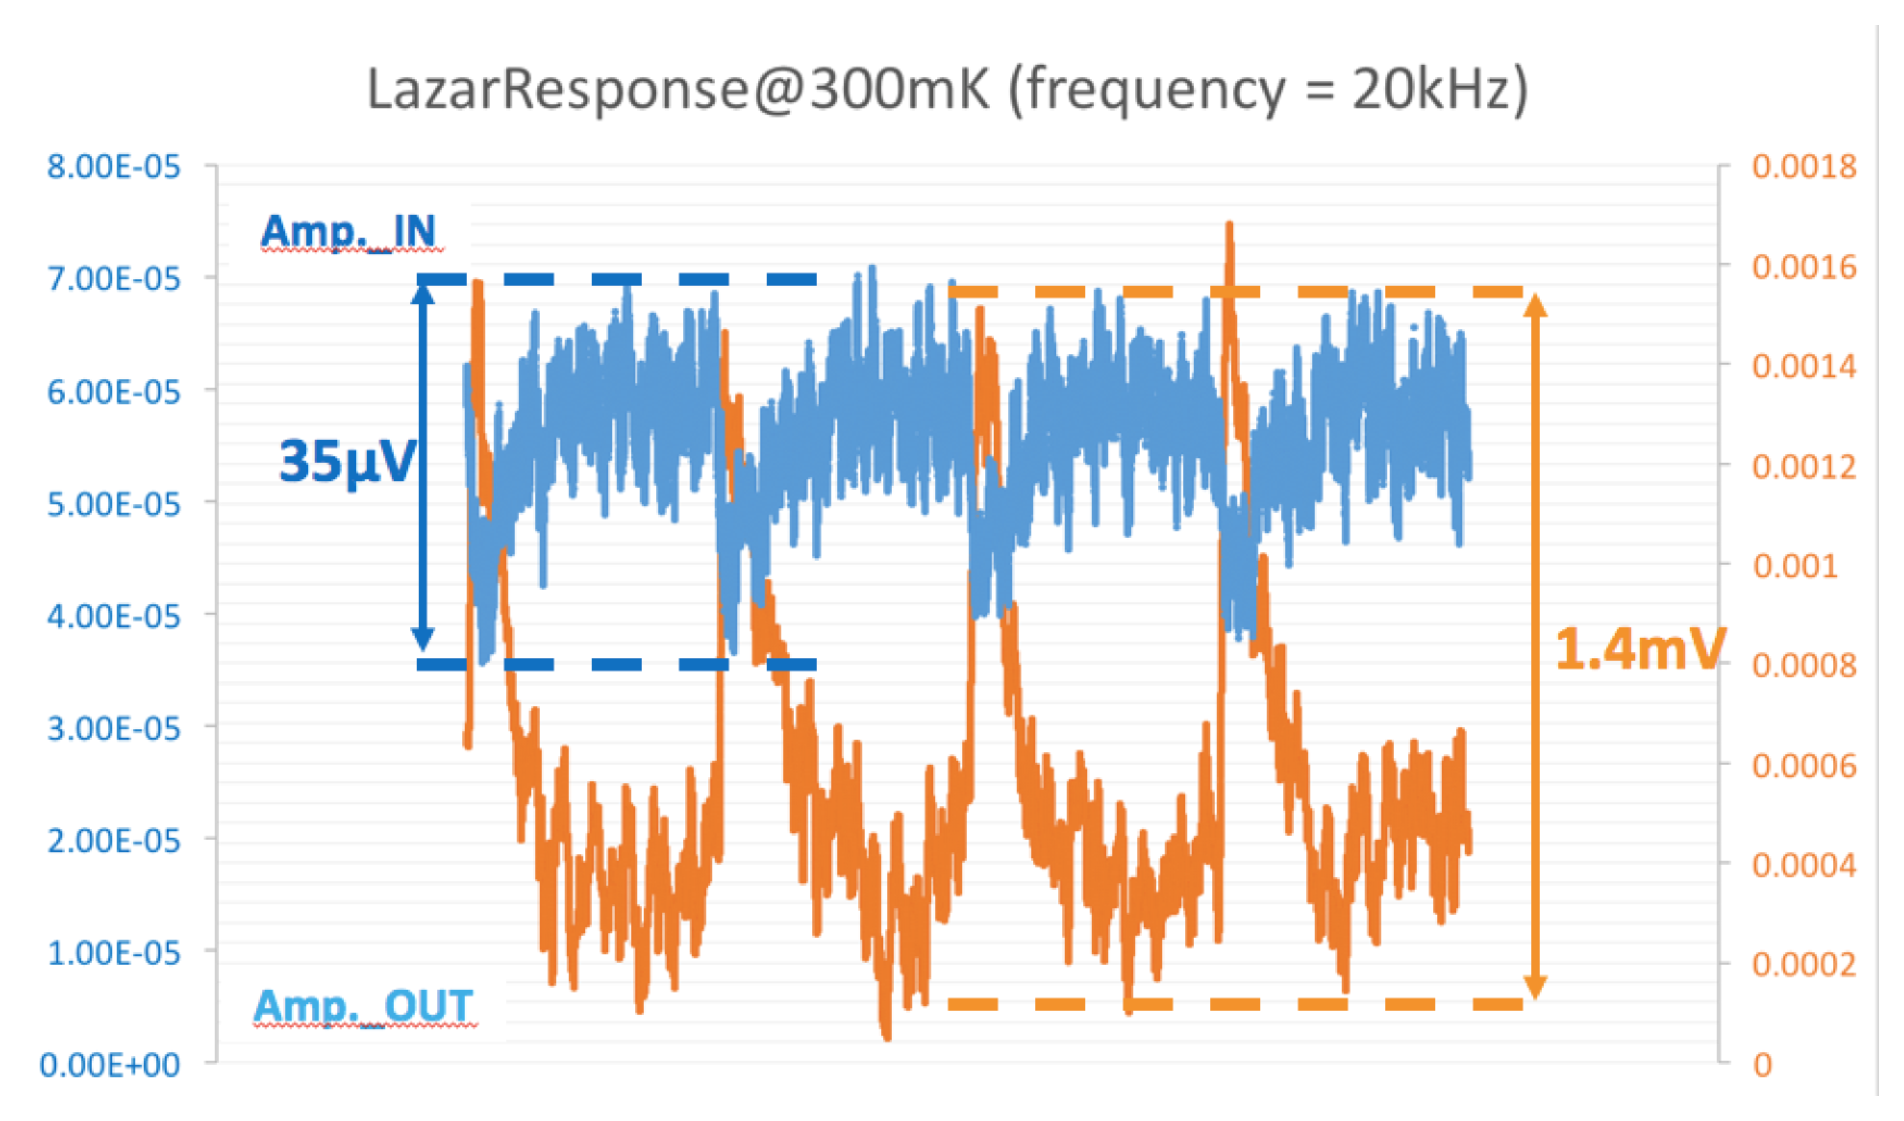
\includegraphics[width=10.0cm]{./Chapter/Chapter4/Picture/STJamp_lazer20k_raw_kakudai.eps}
					\caption{SOI-STJ4を用いたSTJ検出器信号増幅試験(レーザー周波数$f_{\mathrm{lazer}=20\mathrm{kHz}}$\ 直流電源$V_{\mathrm{dc}}=0.43\mathrm{V}$)}
					\label{fig:STJamp_lazer20k_raw_kakudai}
				\end{center}
			\end{figure}
		
			\begin{figure}[htbp]
				\begin{center}
					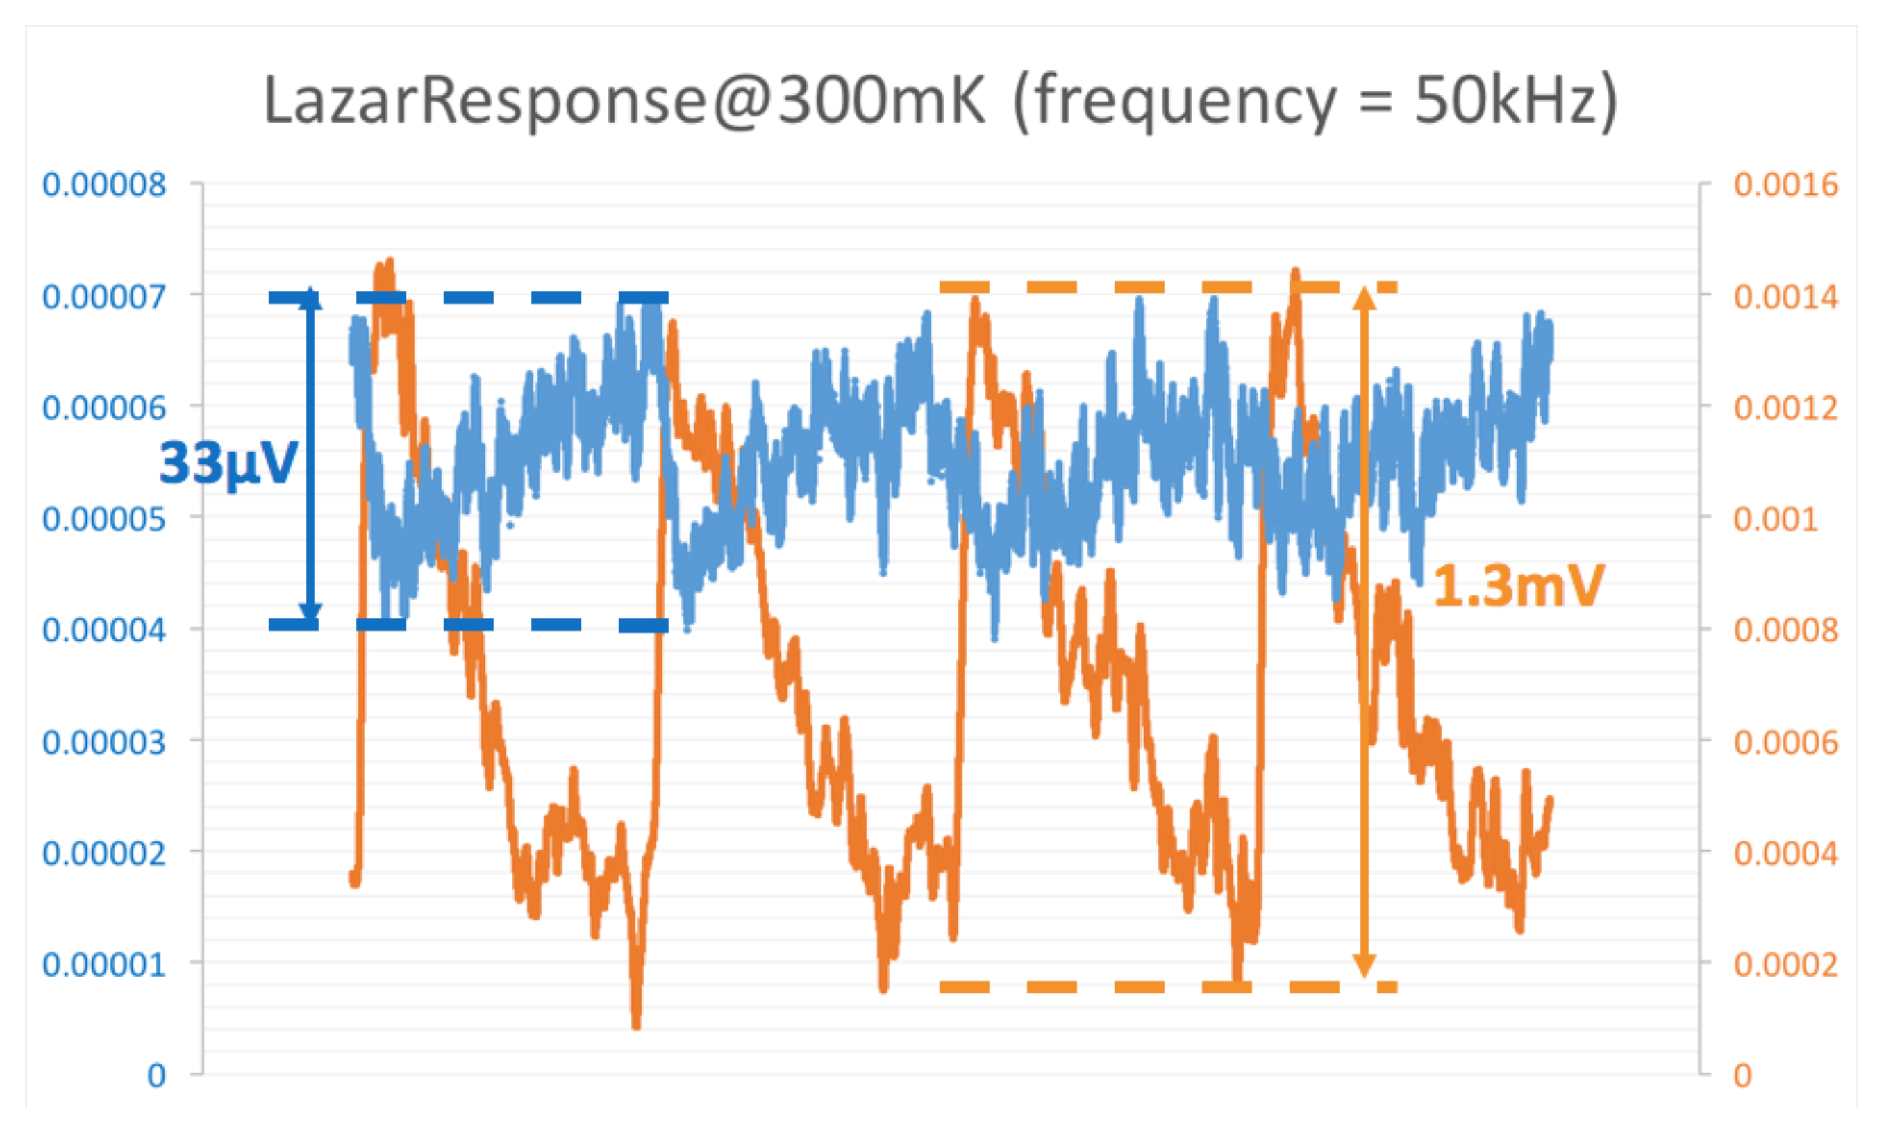
\includegraphics[width=10.0cm]{./Chapter/Chapter4/Picture/STJamp_lazer50k_raw_kakudai.eps}
					\caption{SOI-STJ4を用いたSTJ検出器信号増幅試験(レーザー周波数$f_{\mathrm{lazer}=50\mathrm{kHz}}$\ 直流電源$V_{\mathrm{dc}}=0.43\mathrm{V}$)}
					\label{fig:STJamp_lazer50k_raw_kakudai}
				\end{center}
			\end{figure}
			
			
	
	
	